\section{Einführung in die Integralrechnung}
\label{sec:integralrechnung} % Neues Label zur Unterscheidung
\begin{aufgabenumgebung}{Riemannsummen berechnen}
Gegeben ist die Funktion $f(x) = x+1$.
\begin{enumerate}
    \item Berechne die Untersumme $U_5$ und die Obersumme $O_5$ für das Intervall $[0,5]$ mit $n=5$ Teilintervallen.
    \item Der Graph von $f(x)=x+1$ ist eine Gerade. Der Bereich unter dem Graphen im Intervall $[0,5]$ bildet ein Trapez. Berechne den exakten Flächeninhalt dieses Trapezes mit der geometrischen Formel $A_{Trapez} = \frac{(a+c)}{2} \cdot h$ (wobei $a$ und $c$ die parallelen Seiten sind und $h$ die Höhe).
    \item Vergleiche deine Ergebnisse für $U_5$ und $O_5$ mit dem exakten Flächeninhalt.
    \item Was würde passieren, wenn du $n=10$ oder $n=100$ Teilintervalle wählen würdest? Wie würden sich $U_n$ und $O_n$ verändern?
\end{enumerate}
\end{aufgabenumgebung}

\begin{loesungsumgebung}[loes:riemannsummen-berechnen]{Riemannsummen berechnen}
Gegeben ist die Funktion $f(x) = x+1$ und das Intervall $[0,5]$.

\begin{enumerate}[label=(\alph*)]
    \item \textbf{Berechnung der Untersumme $U_5$ und der Obersumme $O_5$ für $n=5$ Teilintervalle.}
    Die Breite jedes Teilintervalls ist $\Delta x = \frac{b-a}{n} = \frac{5-0}{5} = 1$.
    Die Teilintervalle sind: $[0,1], [1,2], [2,3], [3,4], [4,5]$.
    Die Funktion $f(x)=x+1$ ist eine lineare Funktion mit positiver Steigung ($m=1$), d.h., sie ist im gesamten Intervall $[0,5]$ streng monoton steigend.

    \textbf{Untersumme $U_5$:}
    Da $f(x)$ monoton steigend ist, wird das Minimum in jedem Teilintervall $[x_{i-1}, x_i]$ am linken Rand $x_{i-1}$ angenommen. Die Stützstellen sind $x_0=0, x_1=1, x_2=2, x_3=3, x_4=4$.
    Die Funktionswerte an diesen Stellen sind:
    $f(0) = 0+1 = 1$
    $f(1) = 1+1 = 2$
    $f(2) = 2+1 = 3$
    $f(3) = 3+1 = 4$
    $f(4) = 4+1 = 5$
    Die Untersumme $U_5$ ist:
    $U_5 = \sum_{i=1}^{5} f(x_{i-1}) \cdot \Delta x = (f(0) + f(1) + f(2) + f(3) + f(4)) \cdot 1$
    $U_5 = (1 + 2 + 3 + 4 + 5) \cdot 1 = 15 \cdot 1 = \mathbf{15}$.

    \textbf{Obersumme $O_5$:}
    Da $f(x)$ monoton steigend ist, wird das Maximum in jedem Teilintervall $[x_{i-1}, x_i]$ am rechten Rand $x_i$ angenommen. Die Stützstellen sind $x_1=1, x_2=2, x_3=3, x_4=4, x_5=5$.
    Die Funktionswerte an diesen Stellen sind:
    $f(1) = 1+1 = 2$
    $f(2) = 2+1 = 3$
    $f(3) = 3+1 = 4$
    $f(4) = 4+1 = 5$
    $f(5) = 5+1 = 6$
    Die Obersumme $O_5$ ist:
    $O_5 = \sum_{i=1}^{5} f(x_i) \cdot \Delta x = (f(1) + f(2) + f(3) + f(4) + f(5)) \cdot 1$
    $O_5 = (2 + 3 + 4 + 5 + 6) \cdot 1 = 20 \cdot 1 = \mathbf{20}$.

    \item \textbf{Exakter Flächeninhalt des Trapezes.}
    Der Graph von $f(x)=x+1$ bildet mit der x-Achse und den Geraden $x=0$ und $x=5$ ein Trapez.
    Die parallelen Seiten des Trapezes sind die Funktionswerte an den Intervallgrenzen:
    $a = f(0) = 1$
    $c = f(5) = 5+1 = 6$
    Die Höhe des Trapezes ist die Länge des Intervalls: $h_{Trapez} = 5-0 = 5$.
    Die Trapezformel lautet $A_{Trapez} = \frac{(a+c)}{2} \cdot h_{Trapez}$.
    $A_{Trapez} = \frac{(1+6)}{2} \cdot 5 = \frac{7}{2} \cdot 5 = \frac{35}{2} = \mathbf{17.5}$.

    \item \textbf{Vergleich der Ergebnisse.}
    Wir haben $U_5 = 15$, $O_5 = 20$ und den exakten Flächeninhalt $A = 17.5$.
    Es gilt $\mathbf{15 < 17.5 < 20}$, also $U_5 < A < O_5$.
    Die Untersumme unterschätzt die tatsächliche Fläche, während die Obersumme sie überschätzt. Der exakte Wert liegt erwartungsgemäß zwischen den beiden Summen.

    \item \textbf{Was würde passieren, wenn $n=10$ oder $n=100$ Teilintervalle gewählt würden?}
    Wenn die Anzahl der Teilintervalle $n$ erhöht wird (z.B. auf $n=10$ oder $n=100$), wird die Breite jedes einzelnen Teilintervalls $\Delta x = \frac{b-a}{n}$ kleiner.
    \begin{itemize}
        \item Die Rechtecke, die für die Unter- und Obersumme verwendet werden, passen sich dem tatsächlichen Flächenverlauf unter der Kurve besser an.
        \item Die Untersumme $U_n$ würde \textbf{ansteigen} und sich dem exakten Flächeninhalt $A=17.5$ von unten nähern.
        \item Die Obersumme $O_n$ würde \textbf{absinken} und sich dem exakten Flächeninhalt $A=17.5$ von oben nähern.
        \item Die Differenz zwischen Ober- und Untersumme, $O_n - U_n$, würde kleiner werden.
        \item Im Grenzwert für $n \to \infty$ würden sowohl $U_n$ als auch $O_n$ gegen den exakten Flächeninhalt $A$ konvergieren: $\lim_{n \to \infty} U_n = A$ und $\lim_{n \to \infty} O_n = A$.
    \end{itemize}
    Je mehr Teilintervalle verwendet werden, desto genauer wird die Approximation der Fläche durch die Riemannsummen.
\end{enumerate}

\end{loesungsumgebung}

\begin{aufgabenumgebung}{Stammfunktionen bilden üben}
Bestimme jeweils die Menge aller Stammfunktionen (das unbestimmte Integral) für die folgenden Funktionen:
\begin{enumerate}
    \item $f(x) = x^5$
    \item $g(x) = 12x^3$
    \item $h(x) = 2x^3 - 7x^2 + 4x - 1$
    \item $k(x) = \sqrt{x} + \frac{1}{x^3}$ (Tipp: Erst in Potenzschreibweise $x^n$ umwandeln! $\sqrt{x}=x^{1/2}$ und $\frac{1}{x^3}=x^{-3}$)
    \item $m(t) = at+b$ (wobei $a,b$ Konstanten sind; integriere nach $t$)
    \item $p(x) = (x+1)(x-2)$ (Tipp: Erst ausmultiplizieren!)
\end{enumerate}
Mache bei mindestens zwei Aufgaben die Probe durch Ableiten deiner Stammfunktion.
\end{aufgabenumgebung}
\begin{loesungsumgebung}[loes:stammfunktionen-bilden-ueben]{Stammfunktionen bilden üben}
Wir bestimmen die Menge aller Stammfunktionen $F(x)+C$ (bzw. $M(t)+C$, etc.) für die gegebenen Funktionen.

\begin{enumerate}[label=(\alph*)]
    \item \textbf{Funktion $f(x) = x^5$}
    $$ F(x) = \int x^5 \, dx = \frac{x^{5+1}}{5+1} + C = \mathbf{\frac{1}{6}x^6 + C} $$
    \textit{Probe durch Ableiten:}
    $F'(x) = \frac{d}{dx}\left(\frac{1}{6}x^6 + C\right) = \frac{1}{6} \cdot 6x^{6-1} + 0 = x^5 = f(x)$. Die Probe ist erfolgreich.

    \item \textbf{Funktion $g(x) = 12x^3$}
    $$ G(x) = \int 12x^3 \, dx = 12 \int x^3 \, dx = 12 \cdot \frac{x^{3+1}}{3+1} + C = 12 \cdot \frac{x^4}{4} + C = \mathbf{3x^4 + C} $$

    \item \textbf{Funktion $h(x) = 2x^3 - 7x^2 + 4x - 1$}
    \begin{align*} H(x) &= \int (2x^3 - 7x^2 + 4x - 1) \, dx \\ &= 2\int x^3 \, dx - 7\int x^2 \, dx + 4\int x^1 \, dx - \int 1 \, dx \\ &= 2 \cdot \frac{x^4}{4} - 7 \cdot \frac{x^3}{3} + 4 \cdot \frac{x^2}{2} - 1 \cdot x + C \\ &= \mathbf{\frac{1}{2}x^4 - \frac{7}{3}x^3 + 2x^2 - x + C} \end{align*}
    \textit{Probe durch Ableiten:}
    $H'(x) = \frac{d}{dx}\left(\frac{1}{2}x^4 - \frac{7}{3}x^3 + 2x^2 - x + C\right)$
    $H'(x) = \frac{1}{2} \cdot 4x^3 - \frac{7}{3} \cdot 3x^2 + 2 \cdot 2x - 1 + 0 = 2x^3 - 7x^2 + 4x - 1 = h(x)$. Die Probe ist erfolgreich.

    \item \textbf{Funktion $k(x) = \sqrt{x} + \frac{1}{x^3}$} \\
    Zuerst in Potenzschreibweise umwandeln: $k(x) = x^{1/2} + x^{-3}$.
    \begin{align*} K(x) &= \int (x^{1/2} + x^{-3}) \, dx \\ &= \int x^{1/2} \, dx + \int x^{-3} \, dx \\ &= \frac{x^{\frac{1}{2}+1}}{\frac{1}{2}+1} + \frac{x^{-3+1}}{-3+1} + C \\ &= \frac{x^{3/2}}{3/2} + \frac{x^{-2}}{-2} + C \\ &= \mathbf{\frac{2}{3}x^{3/2} - \frac{1}{2}x^{-2} + C} \end{align*}
    Dies kann auch geschrieben werden als $K(x) = \frac{2}{3}\sqrt{x^3} - \frac{1}{2x^2} + C$.

    \item \textbf{Funktion $m(t) = at+b$} (integriere nach $t$; $a,b$ sind Konstanten)
    \begin{align*} M(t) &= \int (at+b) \, dt \\ &= a \int t^1 \, dt + b \int t^0 \, dt \\ &= a \cdot \frac{t^{1+1}}{1+1} + b \cdot \frac{t^{0+1}}{0+1} + C \\ &= a \frac{t^2}{2} + b t + C \\ &= \mathbf{\frac{1}{2}at^2 + bt + C} \end{align*}

    \item \textbf{Funktion $p(x) = (x+1)(x-2)$} \\
    Zuerst ausmultiplizieren: $p(x) = x^2 - 2x + x - 2 = x^2 - x - 2$.
    \begin{align*} P(x) &= \int (x^2 - x - 2) \, dx \\ &= \int x^2 \, dx - \int x^1 \, dx - \int 2 \, dx \\ &= \frac{x^3}{3} - \frac{x^2}{2} - 2x + C \end{align*}
    Die Menge aller Stammfunktionen ist $\mathbf{P(x) = \frac{1}{3}x^3 - \frac{1}{2}x^2 - 2x + C}$.
\end{enumerate}

\end{loesungsumgebung}



\begin{aufgabenumgebung}{Bestimmte Integrale mit dem HDI berechnen}
Berechne die folgenden bestimmten Integrale mit dem Hauptsatz.
\begin{enumerate}
    \item $\int_{1}^{2} (4x^3 - 6x) \,dx$
    \item $\int_{-1}^{1} (x^2 + 2) \,dx$
    \item $\int_{0}^{4} (\sqrt{x} + 1) \,dx$ (Tipp: $\sqrt{x} = x^{1/2}$)
    \item \textbf{Fläche visualisieren:}
        Die Funktion $f(x) = -x^2 + 4x$ hast du vielleicht schon in früheren Aufgaben skizziert (eine nach unten geöffnete Parabel).
        \begin{itemize}
            \item Berechne die Nullstellen von $f(x)$.
            \item Berechne das bestimmte Integral $\int_{x_1}^{x_2} f(x) \,dx$, wobei $x_1$ und $x_2$ die Nullstellen sind ($x_1 < x_2$).
            \item Was stellt dieser Wert geometrisch dar? Markiere die entsprechende Fläche in einer Skizze des Graphen von $f(x)$.
\begin{center}
    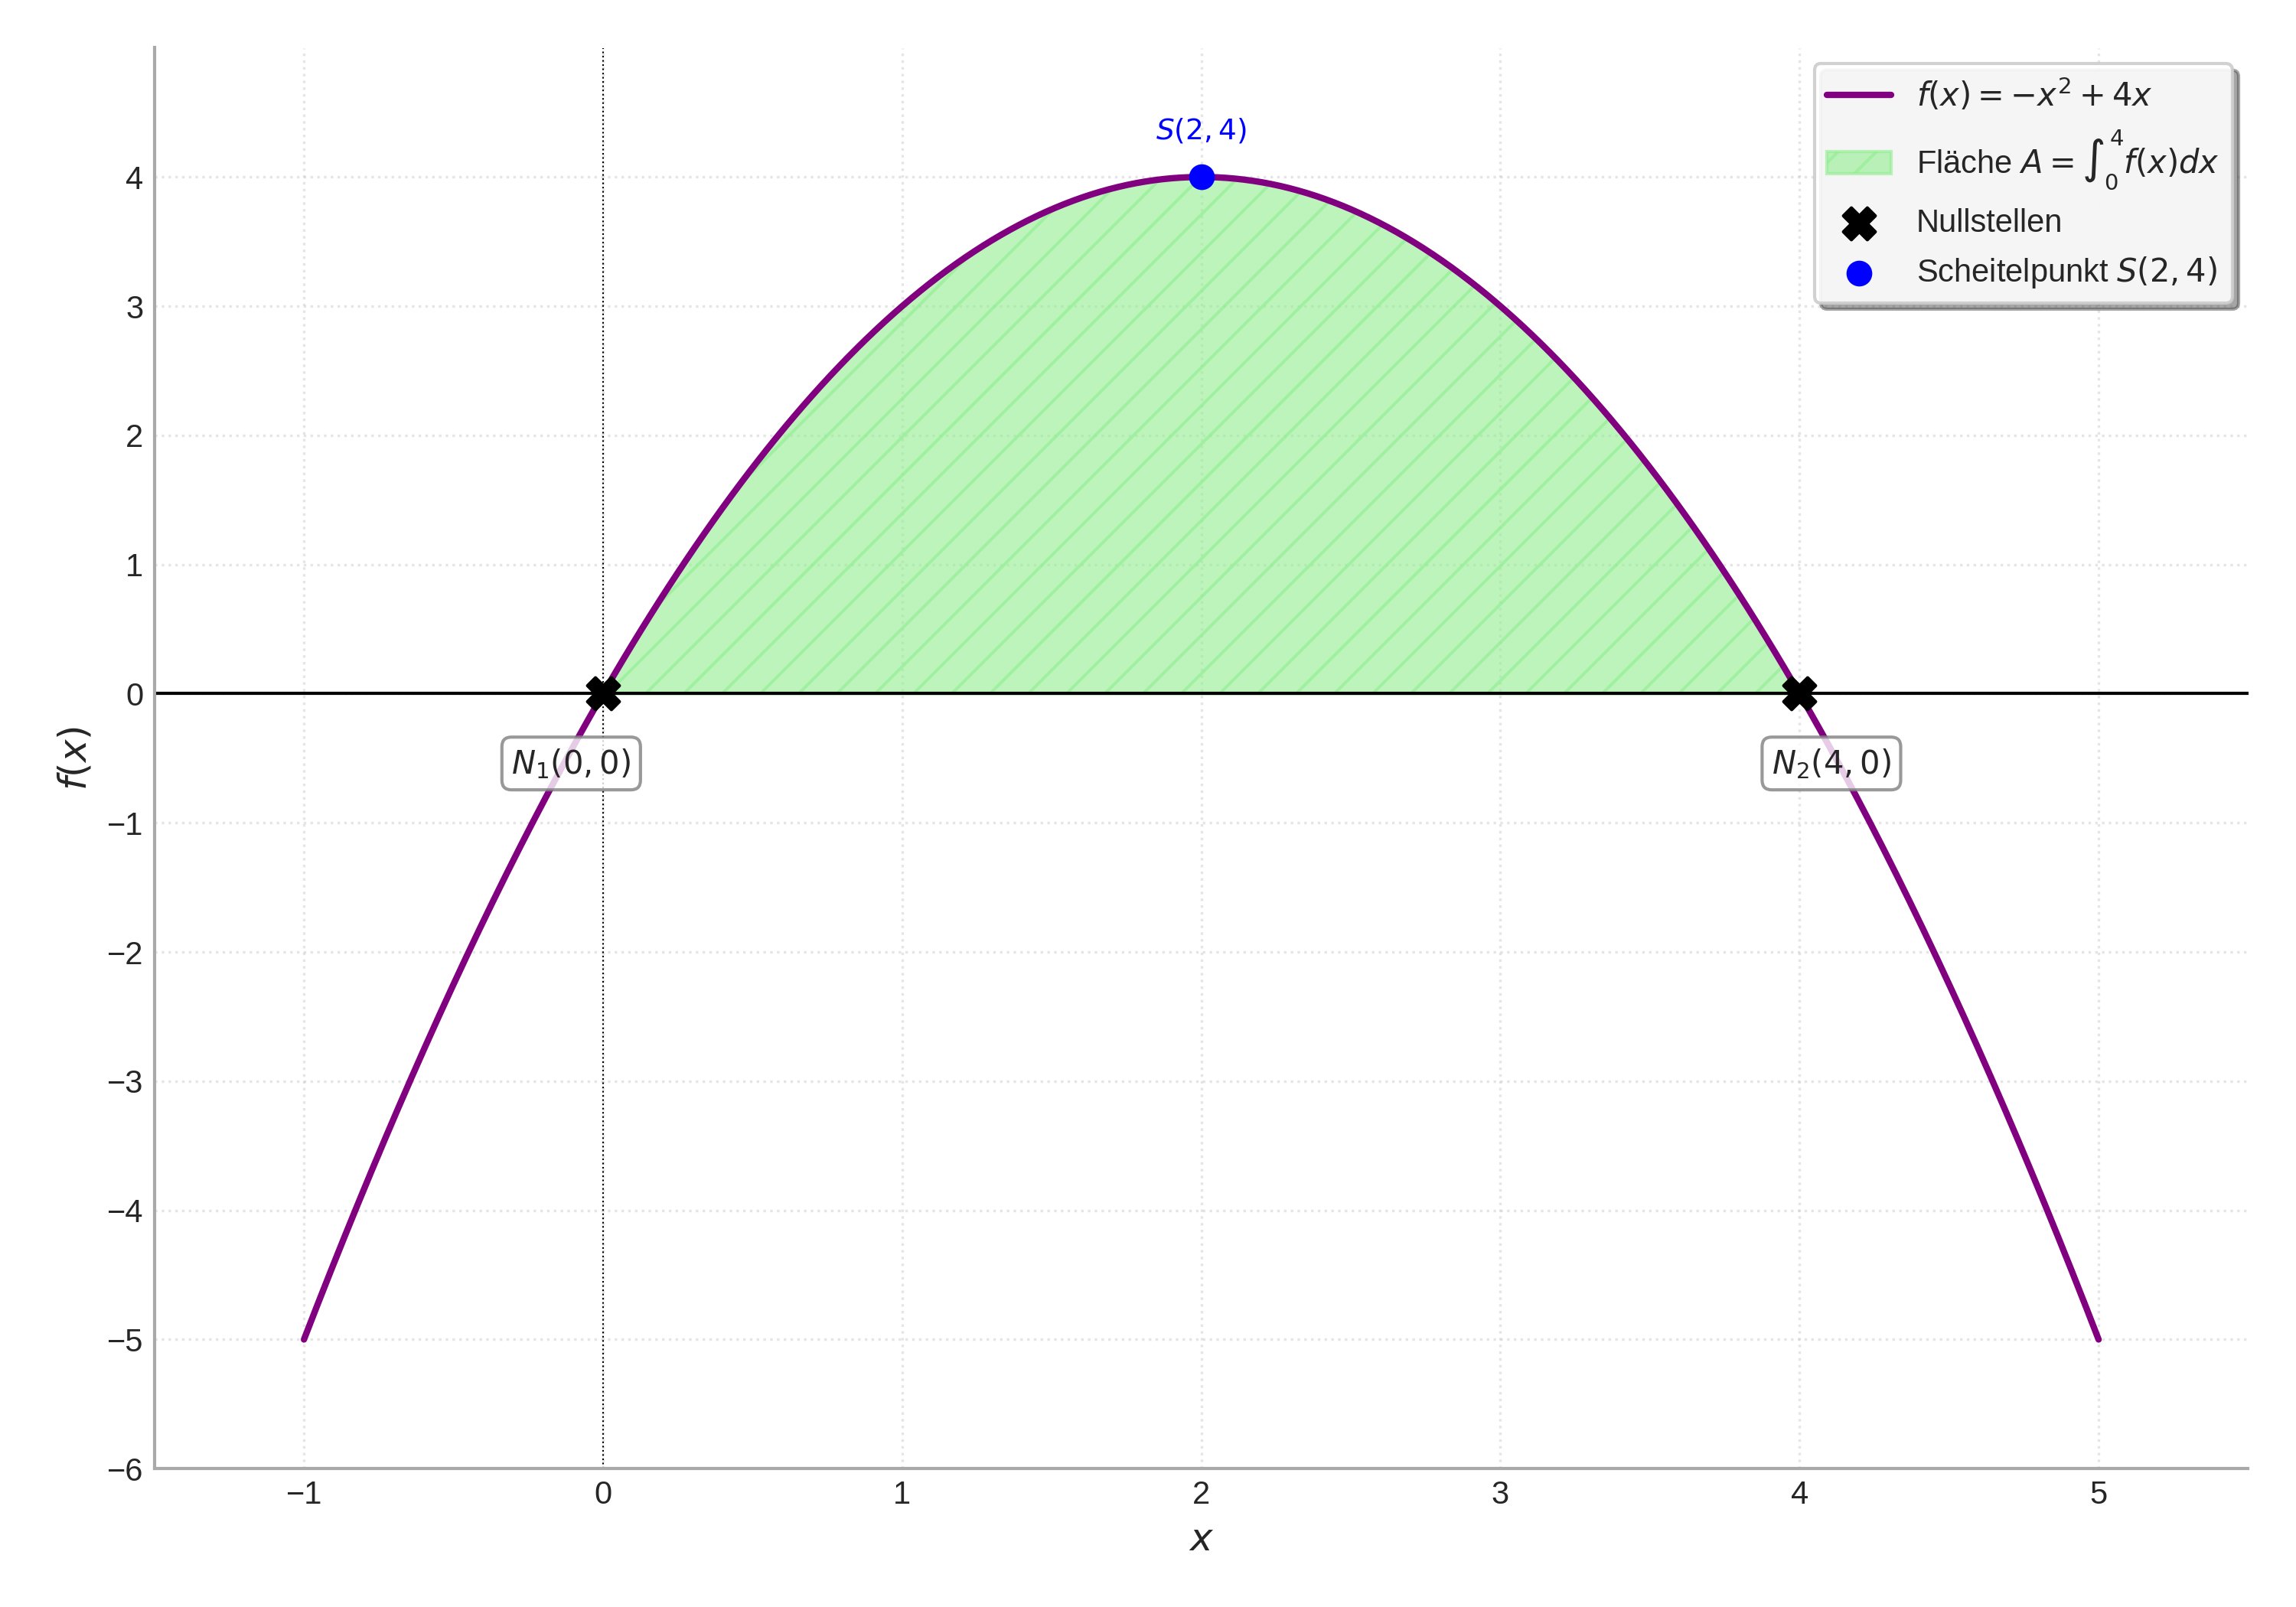
\includegraphics[width=0.5\textwidth]{grafiken/Integral_Flaeche_Parabel.png}
    \captionof{figure}{Fläche unter $f(x)=-x^2+4x$ zwischen den Nullstellen}
    \label{fig:flaeche_parabel}
\end{center}
        \end{itemize}
\end{enumerate}
\end{aufgabenumgebung}


\begin{loesungsumgebung}[loes:bestimmte-integrale-hdi]{Bestimmte Integrale mit dem HDI berechnen}
Wir berechnen die bestimmten Integrale mithilfe des Hauptsatzes der Differential- und Integralrechnung.

\begin{enumerate}[label=(\alph*)]
    \item $\mathbf{\int_{1}^{2} (4x^3 - 6x) \,dx}$
    \begin{itemize}
        \item Zuerst bestimmen wir eine Stammfunktion $F(x)$ von $f(x) = 4x^3 - 6x$:
        $F(x) = \int (4x^3 - 6x) \,dx = 4 \cdot \frac{x^4}{4} - 6 \cdot \frac{x^2}{2} = x^4 - 3x^2$.
        \item Nun wenden wir den HDI an: $\int_{1}^{2} f(x) \,dx = [F(x)]_{1}^{2} = F(2) - F(1)$.
        $F(2) = (2)^4 - 3(2)^2 = 16 - 3(4) = 16 - 12 = 4$.
        $F(1) = (1)^4 - 3(1)^2 = 1 - 3 = -2$.
        \item $\int_{1}^{2} (4x^3 - 6x) \,dx = 4 - (-2) = 4 + 2 = \mathbf{6}$.
    \end{itemize}

    \item $\mathbf{\int_{-1}^{1} (x^2 + 2) \,dx}$
    \begin{itemize}
        \item Stammfunktion $F(x)$ von $f(x) = x^2 + 2$:
        $F(x) = \int (x^2 + 2) \,dx = \frac{x^3}{3} + 2x$.
        \item Anwendung des HDI: $\int_{-1}^{1} f(x) \,dx = [F(x)]_{-1}^{1} = F(1) - F(-1)$.
        $F(1) = \frac{(1)^3}{3} + 2(1) = \frac{1}{3} + 2 = \frac{1}{3} + \frac{6}{3} = \frac{7}{3}$.
        $F(-1) = \frac{(-1)^3}{3} + 2(-1) = -\frac{1}{3} - 2 = -\frac{1}{3} - \frac{6}{3} = -\frac{7}{3}$.
        \item $\int_{-1}^{1} (x^2 + 2) \,dx = \frac{7}{3} - (-\frac{7}{3}) = \frac{7}{3} + \frac{7}{3} = \mathbf{\frac{14}{3}}$.
        \textit{(Hinweis: Da $f(x)=x^2+2$ eine achsensymmetrische Funktion zur y-Achse ist, hätte man auch $2 \cdot \int_{0}^{1} (x^2+2) \,dx$ rechnen können.)}
    \end{itemize}

    \item $\mathbf{\int_{0}^{4} (\sqrt{x} + 1) \,dx}$
    \begin{itemize}
        \item Wir schreiben $\sqrt{x} = x^{1/2}$. Die Funktion ist $f(x) = x^{1/2} + 1$.
        \item Stammfunktion $F(x)$ von $f(x) = x^{1/2} + 1$:
        $F(x) = \int (x^{1/2} + 1) \,dx = \frac{x^{\frac{1}{2}+1}}{\frac{1}{2}+1} + x = \frac{x^{3/2}}{3/2} + x = \frac{2}{3}x^{3/2} + x$.
        \item Anwendung des HDI: $\int_{0}^{4} f(x) \,dx = [F(x)]_{0}^{4} = F(4) - F(0)$.
        $F(4) = \frac{2}{3}(4)^{3/2} + 4 = \frac{2}{3}(\sqrt{4})^3 + 4 = \frac{2}{3}(2)^3 + 4 = \frac{2}{3}(8) + 4 = \frac{16}{3} + \frac{12}{3} = \frac{28}{3}$.
        $F(0) = \frac{2}{3}(0)^{3/2} + 0 = 0$.
        \item $\int_{0}^{4} (\sqrt{x} + 1) \,dx = \frac{28}{3} - 0 = \mathbf{\frac{28}{3}}$.
    \end{itemize}

    \item \textbf{Fläche visualisieren: $f(x) = -x^2 + 4x$}
    \begin{itemize}
        \item \textbf{Nullstellen von $f(x)$:}
        Setze $f(x)=0 \Rightarrow -x^2 + 4x = 0 \Rightarrow -x(x-4) = 0$.
        Die Nullstellen sind $\mathbf{x_1 = 0}$ und $\mathbf{x_2 = 4}$.
        \item \textbf{Bestimmtes Integral $\int_{x_1}^{x_2} f(x) \,dx$ (mit $x_1=0, x_2=4$):}
        Stammfunktion $F(x)$ von $f(x) = -x^2 + 4x$:
        $F(x) = \int (-x^2 + 4x) \,dx = -\frac{x^3}{3} + 4\frac{x^2}{2} = -\frac{1}{3}x^3 + 2x^2$.
        Anwendung des HDI:
        $\int_{0}^{4} (-x^2 + 4x) \,dx = [-\frac{1}{3}x^3 + 2x^2]_{0}^{4}$
        $= \left(-\frac{1}{3}(4)^3 + 2(4)^2\right) - \left(-\frac{1}{3}(0)^3 + 2(0)^2\right)$
        $= \left(-\frac{64}{3} + 2(16)\right) - (0)$
        $= -\frac{64}{3} + 32 = -\frac{64}{3} + \frac{96}{3} = \mathbf{\frac{32}{3}}$.
        \item \textbf{Geometrische Darstellung dieses Werts:}
        Der Wert $\frac{32}{3}$ (ca. $10.67$) stellt den \textbf{Flächeninhalt} dar, der vom Graphen der Funktion $f(x)=-x^2+4x$ und der x-Achse im Intervall $[0,4]$ eingeschlossen wird.
        Da die Funktion $f(x)$ eine nach unten geöffnete Parabel mit Nullstellen bei $x=0$ und $x=4$ ist, verläuft der Graph für $x \in (0,4)$ oberhalb der x-Achse. Daher ist das bestimmte Integral in diesen Grenzen positiv und entspricht direkt dem Flächeninhalt dieses Parabelsegments.
        In der Abbildung \ref{fig:flaeche_parabel} ist diese Fläche unter dem Graphen von $f(x)$ zwischen den Nullstellen $x=0$ und $x=4$ markiert.
    \end{itemize}
\end{enumerate}

\end{loesungsumgebung}


\begin{aufgabenumgebung}{Flächenberechnung mit Nullstellen im Intervall}
Berechne den Inhalt der Fläche, die vom Graphen der Funktion $f(x) = x^3 - x$ und der x-Achse im Intervall $[-2, 2]$ eingeschlossen wird.
\end{aufgabenumgebung}

\begin{loesungsumgebung}[loes:flaeche-mit-nullstellen-intervall]{Flächenberechnung mit Nullstellen im Intervall}
Gegeben ist die Funktion $f(x) = x^3 - x$ und das Intervall $[-2, 2]$. Wir folgen den Schritten aus dem Tipp:

\begin{enumerate}
    \item \textbf{Verlauf anhand von Symmetrie und Nullstellen überlegen:}
    \begin{itemize}
        \item \textbf{Nullstellen:} $f(x) = x^3 - x = x(x^2-1) = x(x-1)(x+1)$.
        Die Nullstellen sind $x_1 = -1$, $x_2 = 0$ und $x_3 = 1$. Alle diese Nullstellen liegen im Intervall $[-2, 2]$.
        \item \textbf{Symmetrie:} $f(-x) = (-x)^3 - (-x) = -x^3 + x = -(x^3-x) = -f(x)$.
        Die Funktion ist punktsymmetrisch zum Ursprung.
        \item \textbf{Globalverhalten:} Der Leitterm ist $x^3$. Für $x \to \infty$ geht $f(x) \to \infty$, und für $x \to -\infty$ geht $f(x) \to -\infty$.
        Der Graph kommt also von links unten, schneidet die x-Achse bei $-1, 0, 1$ und geht nach rechts oben.
    \end{itemize}

    \item \textbf{Alle Nullstellen von $f(x)$ (bereits in Schritt 1 erledigt):}
    Die Nullstellen sind $\mathbf{x_1 = -1}$, $\mathbf{x_2 = 0}$, $\mathbf{x_3 = 1}$.

    \item \textbf{Bestimmung der Teilintervalle und Vorzeichen von $f(x)$ im Intervall $[-2, 2]$:}
    Die Nullstellen $-1, 0, 1$ unterteilen das Intervall $[-2, 2]$ in die folgenden Teilintervalle:
    $[-2, -1]$, $[-1, 0]$, $[0, 1]$ und $[1, 2]$.
    Wir bestimmen das Vorzeichen von $f(x) = x(x-1)(x+1)$ in diesen Intervallen:
    \begin{itemize}
        \item Intervall $[-2, -1]$: Wähle z.B. $x=-1.5$.
        $f(-1.5) = (-1.5)(-1.5-1)(-1.5+1) = (-1.5)(-2.5)(-0.5) < 0$. Also $f(x) \le 0$.
        \item Intervall $[-1, 0]$: Wähle z.B. $x=-0.5$.
        $f(-0.5) = (-0.5)(-0.5-1)(-0.5+1) = (-0.5)(-1.5)(0.5) > 0$. Also $f(x) \ge 0$.
        \item Intervall $[0, 1]$: Wähle z.B. $x=0.5$.
        $f(0.5) = (0.5)(0.5-1)(0.5+1) = (0.5)(-0.5)(1.5) < 0$. Also $f(x) \le 0$.
        \item Intervall $[1, 2]$: Wähle z.B. $x=1.5$.
        $f(1.5) = (1.5)(1.5-1)(1.5+1) = (1.5)(0.5)(2.5) > 0$. Also $f(x) \ge 0$.
    \end{itemize}

    \item \textbf{Berechnung der bestimmten Integrale und Addition der Beträge:}
    Die Gesamtfläche $A$ ist die Summe der Beträge der Integrale über die Teilintervalle:
    $A = \left| \int_{-2}^{-1} (x^3-x) \,dx \right| + \left| \int_{-1}^{0} (x^3-x) \,dx \right| + \left| \int_{0}^{1} (x^3-x) \,dx \right| + \left| \int_{1}^{2} (x^3-x) \,dx \right|$.
    Eine Stammfunktion von $f(x) = x^3-x$ ist $F(x) = \frac{1}{4}x^4 - \frac{1}{2}x^2$.
    \begin{itemize}
        \item $\int_{-2}^{-1} (x^3-x) \,dx = [F(x)]_{-2}^{-1} = F(-1) - F(-2)$
        $F(-1) = \frac{1}{4}(-1)^4 - \frac{1}{2}(-1)^2 = \frac{1}{4} - \frac{1}{2} = -\frac{1}{4}$.
        $F(-2) = \frac{1}{4}(-2)^4 - \frac{1}{2}(-2)^2 = \frac{16}{4} - \frac{4}{2} = 4 - 2 = 2$.
        Integral $I_1 = -\frac{1}{4} - 2 = -\frac{9}{4}$. Betrag: $|I_1| = \frac{9}{4}$.

        \item $\int_{-1}^{0} (x^3-x) \,dx = [F(x)]_{-1}^{0} = F(0) - F(-1)$
        $F(0) = 0$.
        Integral $I_2 = 0 - (-\frac{1}{4}) = \frac{1}{4}$. Betrag: $|I_2| = \frac{1}{4}$.

        \item $\int_{0}^{1} (x^3-x) \,dx = [F(x)]_{0}^{1} = F(1) - F(0)$
        $F(1) = \frac{1}{4}(1)^4 - \frac{1}{2}(1)^2 = \frac{1}{4} - \frac{1}{2} = -\frac{1}{4}$.
        Integral $I_3 = -\frac{1}{4} - 0 = -\frac{1}{4}$. Betrag: $|I_3| = \frac{1}{4}$.

        \item $\int_{1}^{2} (x^3-x) \,dx = [F(x)]_{1}^{2} = F(2) - F(1)$
        $F(2) = \frac{1}{4}(2)^4 - \frac{1}{2}(2)^2 = 4 - 2 = 2$.
        Integral $I_4 = 2 - (-\frac{1}{4}) = \frac{9}{4}$. Betrag: $|I_4| = \frac{9}{4}$.
    \end{itemize}
    Der gesamte Flächeninhalt ist:
    $A = |I_1| + |I_2| + |I_3| + |I_4| = \frac{9}{4} + \frac{1}{4} + \frac{1}{4} + \frac{9}{4} = \frac{20}{4} = \mathbf{5}$ Flächeneinheiten.

    \textit{Alternative Berechnung unter Nutzung der Punktsymmetrie:}
    Da $f(x)$ punktsymmetrisch zum Ursprung ist, gilt $\left| \int_{-a}^{-b} f(x) \,dx \right| = \left| \int_{b}^{a} f(x) \,dx \right|$ und $\left| \int_{-b}^{0} f(x) \,dx \right| = \left| \int_{0}^{b} f(x) \,dx \right|$.
    Somit ist die Fläche im Intervall $[-2,0]$ gleich der Fläche im Intervall $[0,2]$.
    $A = 2 \cdot \left( \left| \int_{0}^{1} (x^3-x) \,dx \right| + \left| \int_{1}^{2} (x^3-x) \,dx \right| \right)$
    $A = 2 \cdot \left( |-\frac{1}{4}| + |\frac{9}{4}| \right) = 2 \cdot \left( \frac{1}{4} + \frac{9}{4} \right) = 2 \cdot \frac{10}{4} = 2 \cdot \frac{5}{2} = 5$.
\end{enumerate}

\end{loesungsumgebung}


\begin{aufgabenumgebung}{Symmetrie beim Integrieren anwenden}
Berechne die folgenden bestimmten Integrale. Nutze Symmetrieeigenschaften, wenn möglich, um die Rechnung zu vereinfachen.
\begin{enumerate}
    \item $\int_{-5}^{5} (x^5 - 2x^3 + x) \,dx$
    \item $\int_{-1}^{1} (x^4 + 3x^2 - 1) \,dx$
    \item $\int_{-\pi}^{\pi} \sin(x) \,dx$ (Du weißt vielleicht schon, dass $\sin(x)$ punktsymmetrisch ist. Die Stammfunktion von $\sin(x)$ ist $-\cos(x)$.)
\end{enumerate}
\end{aufgabenumgebung}


\begin{loesungsumgebung}[loes:symmetrie-integrieren]{Symmetrie beim Integrieren anwenden}
Wir berechnen die bestimmten Integrale und nutzen dabei Symmetrieeigenschaften zur Vereinfachung, falls möglich.

\begin{enumerate}[label=(\alph*)]
    \item $\mathbf{\int_{-5}^{5} (x^5 - 2x^3 + x) \,dx}$
    \begin{itemize}
        \item \textbf{Symmetrieuntersuchung des Integranden:}
        Sei $f(x) = x^5 - 2x^3 + x$.
        $f(-x) = (-x)^5 - 2(-x)^3 + (-x) = -x^5 - 2(-x^3) - x = -x^5 + 2x^3 - x = -(x^5 - 2x^3 + x) = -f(x)$.
        Da $f(-x) = -f(x)$, ist $f(x)$ eine \textbf{ungerade Funktion} (punktsymmetrisch zum Ursprung).
        \item \textbf{Anwendung der Symmetrieeigenschaft:}
        Für eine ungerade Funktion, die über ein zum Ursprung symmetrisches Intervall $[-a, a]$ integriert wird, ist der Wert des bestimmten Integrals Null.
        $$ \int_{-5}^{5} (x^5 - 2x^3 + x) \,dx = \mathbf{0} $$
        \item \textit{Zur Kontrolle (direkte Berechnung):}
        Eine Stammfunktion ist $F(x) = \frac{1}{6}x^6 - \frac{1}{2}x^4 + \frac{1}{2}x^2$.
        $F(5) = \frac{1}{6}(5)^6 - \frac{1}{2}(5)^4 + \frac{1}{2}(5)^2 = \frac{15625}{6} - \frac{625}{2} + \frac{25}{2} = \frac{15625 - 1875 + 75}{6} = \frac{13825}{6}$.
        $F(-5) = \frac{1}{6}(-5)^6 - \frac{1}{2}(-5)^4 + \frac{1}{2}(-5)^2 = \frac{15625}{6} - \frac{625}{2} + \frac{25}{2} = F(5)$.
        $\int_{-5}^{5} f(x) \,dx = F(5) - F(-5) = F(5) - F(5) = 0$.
    \end{itemize}

    \item $\mathbf{\int_{-1}^{1} (x^4 + 3x^2 - 1) \,dx}$
    \begin{itemize}
        \item \textbf{Symmetrieuntersuchung des Integranden:}
        Sei $f(x) = x^4 + 3x^2 - 1$.
        $f(-x) = (-x)^4 + 3(-x)^2 - 1 = x^4 + 3x^2 - 1 = f(x)$.
        Da $f(-x) = f(x)$, ist $f(x)$ eine \textbf{gerade Funktion} (achsensymmetrisch zur y-Achse).
        \item \textbf{Anwendung der Symmetrieeigenschaft:}
        Für eine gerade Funktion gilt $\int_{-a}^{a} f(x) \,dx = 2 \int_{0}^{a} f(x) \,dx$.
        $$ \int_{-1}^{1} (x^4 + 3x^2 - 1) \,dx = 2 \int_{0}^{1} (x^4 + 3x^2 - 1) \,dx $$
        \item \textbf{Berechnung:}
        Eine Stammfunktion von $x^4 + 3x^2 - 1$ ist $F(x) = \frac{x^5}{5} + x^3 - x$.
        \begin{align*}
        2 \int_{0}^{1} (x^4 + 3x^2 - 1) \,dx &= 2 \left[ \frac{x^5}{5} + x^3 - x \right]_{0}^{1} \\
        &= 2 \left( \left(\frac{1^5}{5} + 1^3 - 1\right) - \left(\frac{0^5}{5} + 0^3 - 0\right) \right) \\
        &= 2 \left( \left(\frac{1}{5} + 1 - 1\right) - 0 \right) \\
        &= 2 \left( \frac{1}{5} \right) = \mathbf{\frac{2}{5}}
        \end{align*}
    \end{itemize}

    \item $\mathbf{\int_{-\pi}^{\pi} \sin(x) \,dx}$
    \begin{itemize}
        \item \textbf{Symmetrieuntersuchung des Integranden:}
        Sei $f(x) = \sin(x)$. Es ist bekannt (und aus dem Tipp entnehmbar), dass $\sin(x)$ eine ungerade Funktion ist: $\sin(-x) = -\sin(x)$.
        \item \textbf{Anwendung der Symmetrieeigenschaft:}
        Da $\sin(x)$ eine ungerade Funktion ist und über ein zum Ursprung symmetrisches Intervall $[-\pi, \pi]$ integriert wird, ist der Wert des bestimmten Integrals Null.
        $$ \int_{-\pi}^{\pi} \sin(x) \,dx = \mathbf{0} $$
        \item \textit{Zur Kontrolle (direkte Berechnung mit Stammfunktion $F(x)=-\cos(x)$):}
        \begin{align*}
        \int_{-\pi}^{\pi} \sin(x) \,dx &= [-\cos(x)]_{-\pi}^{\pi} \\
        &= (-\cos(\pi)) - (-\cos(-\pi)) \\
        &= (-(-1)) - (-(-1)) \quad (\text{da } \cos(\pi)=-1 \text{ und } \cos(-\pi)=\cos(\pi)=-1) \\
        &= (1) - (1) = 0
        \end{align*}
    \end{itemize}
\end{enumerate}

\end{loesungsumgebung}

\begin{aufgabenumgebung}{Fläche zwischen zwei Kurven}
Die Graphen der Funktionen $f(x) = -x^2 + 4x + 1$ und $g(x) = x^2 - 2x + 1$ schließen eine Fläche ein.
\begin{enumerate}
    \item \textbf{Schnittpunkte bestimmen:} Berechne die x-Koordinaten der Schnittpunkte der beiden Graphen, indem du $f(x) = g(x)$ setzt und die entstehende Gleichung löst. Diese Schnittpunkte sind deine Integrationsgrenzen $a$ und $b$.
    \item \textbf{Welche Funktion liegt oben?} Bestimme, welche der beiden Funktionen im Intervall $[a,b]$ die größeren Funktionswerte hat (also 'oben' liegt). Du kannst dies tun, indem du einen Testwert aus dem Intervall $(a,b)$ in beide Funktionen einsetzt oder die Graphen skizzierst.
    \item \textbf{Differenzfunktion bilden:} Bilde die Differenzfunktion $d(x) = \text{obere Funktion} - \text{untere Funktion}$.
    \item \textbf{Flächeninhalt berechnen:} Berechne den Flächeninhalt $A = \int_a^b d(x) \,dx$.
    \item \textbf{Skizze:} Skizziere beide Parabeln und die eingeschlossene Fläche in ein Koordinatensystem.
\end{enumerate}
\begin{merksatzumgebung}{Fläche zwischen zwei Graphen}
Den Flächeninhalt $A$ zwischen den Graphen zweier Funktionen $f(x)$ und $g(x)$ im Intervall $[a,b]$, wobei $f(x) \ge g(x)$ für alle $x \in [a,b]$ gilt (d.h. $f(x)$ ist die obere Funktion), berechnet man mit:
\[ A = \int_a^b (f(x) - g(x)) \,dx \]
Wenn nicht klar ist, welche Funktion oben liegt, oder wenn sich die obere Funktion ändert, muss man das Intervall entsprechend aufteilen und/oder den Betrag der Differenz integrieren: $A = \int_a^b |f(x) - g(x)| \,dx$.
\end{merksatzumgebung}
\begin{center}
    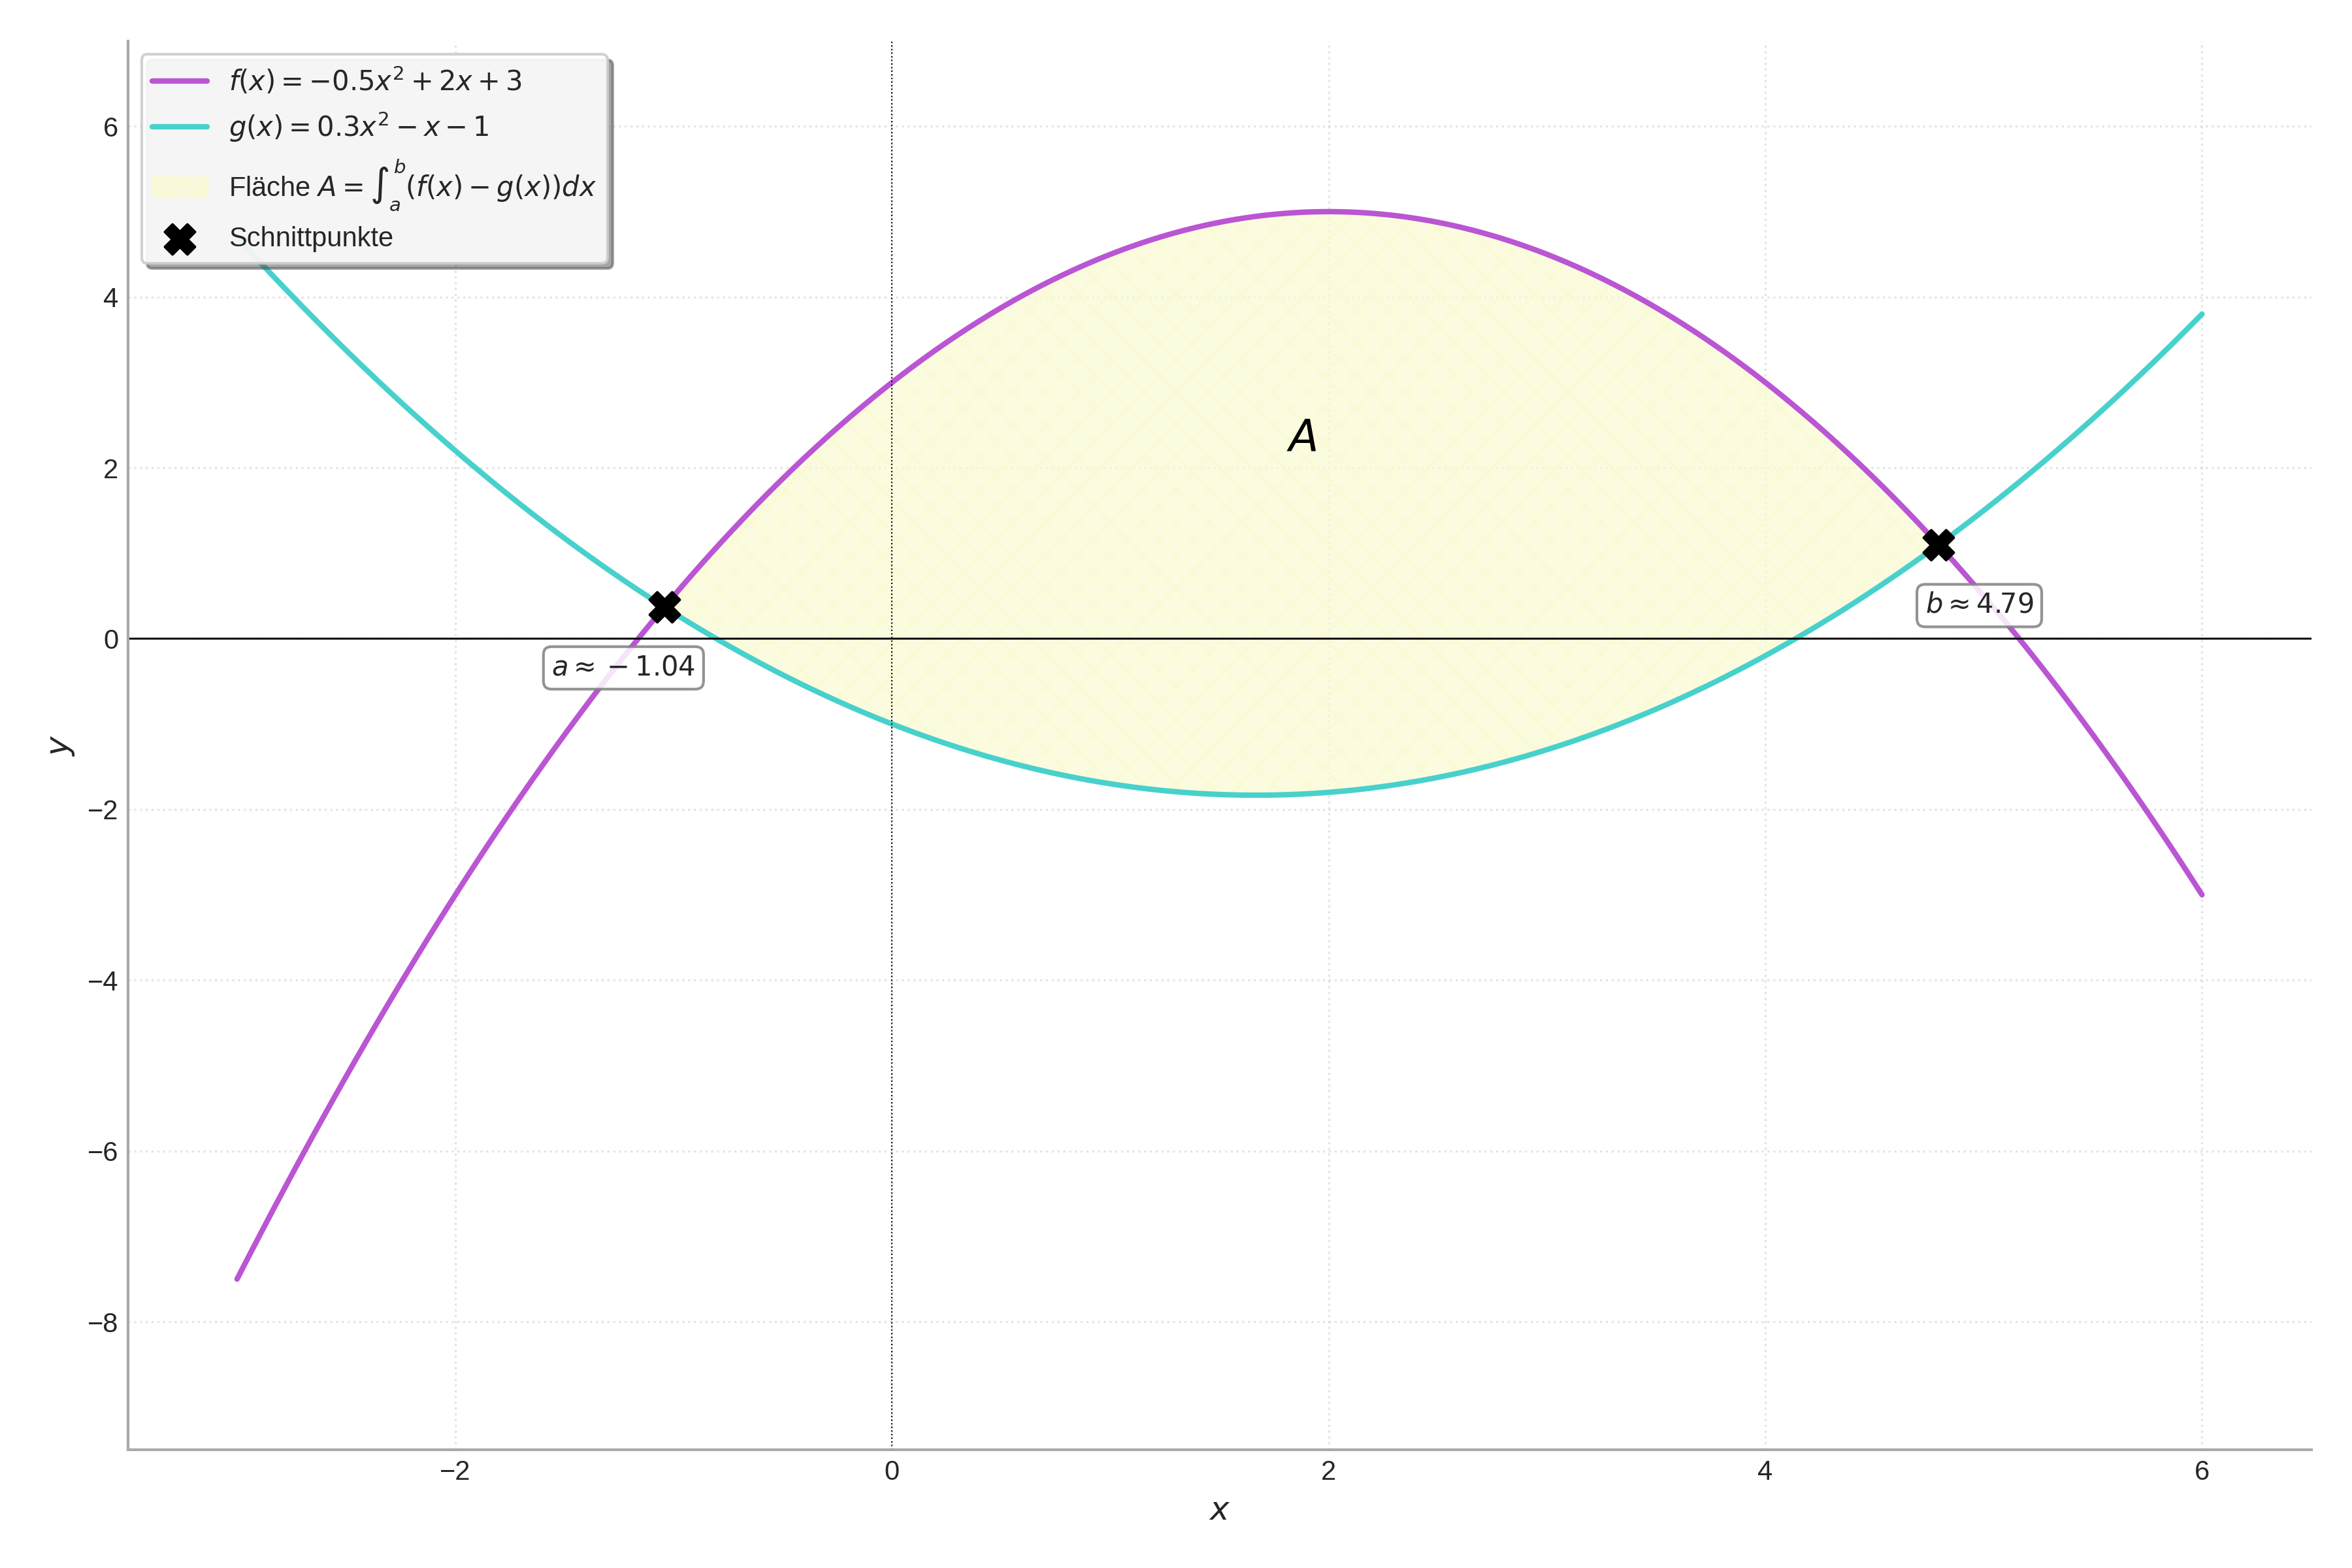
\includegraphics[width=0.8\textwidth]{grafiken/Integral_Flaeche_zwischen_Kurven.png}
    \captionof{figure}{Fläche zwischen den Graphen von $f(x)$ und $g(x)$}
    \label{fig:flaeche_zwischen_kurven}
\end{center}
\end{aufgabenumgebung}

\begin{loesungsumgebung}[loes:flaeche-zwischen-kurven]{Fläche zwischen zwei Kurven}
Gegeben sind die Funktionen $f(x) = -x^2 + 4x + 1$ und $g(x) = x^2 - 2x + 1$.

\begin{enumerate}[label=(\alph*)]
    \item \textbf{Schnittpunkte bestimmen:}
    Wir setzen $f(x) = g(x)$, um die x-Koordinaten der Schnittpunkte zu finden:
    $$ -x^2 + 4x + 1 = x^2 - 2x + 1 $$
    Wir bringen alle Terme auf eine Seite:
    $$ 0 = x^2 - 2x + 1 - (-x^2 + 4x + 1) $$
    $$ 0 = x^2 - 2x + 1 + x^2 - 4x - 1 $$
    $$ 0 = 2x^2 - 6x $$
    Diese quadratische Gleichung lösen wir durch Ausklammern:
    $$ 2x(x-3) = 0 $$
    Die Lösungen (x-Koordinaten der Schnittpunkte) sind:
    $x_1 = 0$ und $x_2 = 3$.
    Dies sind unsere Integrationsgrenzen $a=0$ und $b=3$.

    \item \textbf{Welche Funktion liegt oben im Intervall $[0,3]$?}
    Um festzustellen, welche Funktion im Intervall $(0,3)$ die größeren Funktionswerte hat, wählen wir einen Testwert aus diesem Intervall, z.B. $x=1$:
    $f(1) = -(1)^2 + 4(1) + 1 = -1 + 4 + 1 = 4$.
    $g(1) = (1)^2 - 2(1) + 1 = 1 - 2 + 1 = 0$.
    Da $f(1) = 4 > g(1) = 0$, liegt der Graph von $f(x)$ im Intervall $(0,3)$ oberhalb des Graphen von $g(x)$.

    \item \textbf{Differenzfunktion bilden:}
    Die Differenzfunktion $d(x)$ ist 'obere Funktion - untere Funktion':
    $d(x) = f(x) - g(x) = (-x^2 + 4x + 1) - (x^2 - 2x + 1)$
    $d(x) = -x^2 + 4x + 1 - x^2 + 2x - 1$
    $\mathbf{d(x) = -2x^2 + 6x}$.

    \item \textbf{Flächeninhalt berechnen:}
    Der Flächeninhalt $A$ ist das bestimmte Integral der Differenzfunktion $d(x)$ von $a=0$ bis $b=3$:
    $$ A = \int_0^3 (-2x^2 + 6x) \,dx $$
    Zuerst bestimmen wir eine Stammfunktion $D(x)$ von $d(x)$:
    $D(x) = \int (-2x^2 + 6x) \,dx = -2 \cdot \frac{x^3}{3} + 6 \cdot \frac{x^2}{2} = -\frac{2}{3}x^3 + 3x^2$.
    Nun wenden wir den Hauptsatz der Differential- und Integralrechnung an:
    \begin{align*}
    A &= \left[ -\frac{2}{3}x^3 + 3x^2 \right]_0^3 \\
      &= \left( -\frac{2}{3}(3)^3 + 3(3)^2 \right) - \left( -\frac{2}{3}(0)^3 + 3(0)^2 \right) \\
      &= \left( -\frac{2}{3}(27) + 3(9) \right) - (0) \\
      &= (-2 \cdot 9 + 27) - 0 \\
      &= -18 + 27 \\
      &= \mathbf{9}
    \end{align*}
    Der Flächeninhalt zwischen den beiden Kurven beträgt $9$ Flächeneinheiten.

    \item \textbf{Skizze:}
    Die Abbildung \ref{fig:flaeche_zwischen_kurven} im Aufgabentext visualisiert eine solche Situation. Für die gegebenen Funktionen:
    \begin{itemize}
        \item $f(x) = -x^2 + 4x + 1$ ist eine nach unten geöffnete Parabel. Ihr Scheitelpunkt ist bei $x_S = -4/(2(-1)) = 2$, $f(2) = -4+8+1=5$, also $S_f(2|5)$. Die y-Achse wird bei $(0|1)$ geschnitten.
        \item $g(x) = x^2 - 2x + 1 = (x-1)^2$ ist eine nach oben geöffnete Parabel. Ihr Scheitelpunkt ist bei $(1|0)$ (was auch eine doppelte Nullstelle ist). Die y-Achse wird bei $(0|1)$ geschnitten.
        \item Die Schnittpunkte der Graphen sind $S_1(0|1)$ (da $f(0)=1, g(0)=1$) und $S_2(3|4)$ (da $f(3)=-9+12+1=4, g(3)=9-6+1=4$).
        \item Die Skizze würde diese beiden Parabeln zeigen, die sich bei $(0|1)$ und $(3|4)$ schneiden. Die Fläche zwischen den Kurven in diesem Intervall $[0,3]$ wäre markiert, wobei der Graph von $f(x)$ oberhalb des Graphen von $g(x)$ verläuft.
    \end{itemize}
\end{enumerate}

\end{loesungsumgebung}

\begin{aufgabenumgebung}{Der Mittelwert einer Funktion}
Manchmal möchte man nicht den Gesamtwert (wie die Gesamtfläche oder den Gesamtweg), sondern einen Durchschnittswert einer Größe über ein Intervall bestimmen. Die Integralrechnung hilft auch hier!

\begin{merksatzumgebung}{Mittelwert einer Funktion}
Der \textbf{Mittelwert $\mu$} einer stetigen Funktion $f(x)$ im Intervall $[a,b]$ (mit $a<b$) ist definiert als:
\[ \mu = \frac{1}{b-a} \int_a^b f(x) \,dx \]
\textit{Anschauliche Deutung:} Der Mittelwert $\mu$ ist die Höhe eines Rechtecks mit der Breite $(b-a)$, dessen Flächeninhalt gleich dem Flächeninhalt unter dem Graphen von $f(x)$ im Intervall $[a,b]$ ist. Also: $\mu \cdot (b-a) = \int_a^b f(x) \,dx$.
\end{merksatzumgebung}

\textbf{Aufgabe:}
Ein Tag hat vereinfacht 12 Stunden Helligkeit (von $t=0$ bis $t=12$). Die Temperatur $T$ (in °C) an diesem Tag kann durch die Funktion $T(t) = -0.5t^2 + 6t + 5$ modelliert werden.
\begin{enumerate}
    \item Skizziere den Graphen der Temperaturfunktion im Intervall $[0,12]$.
    \item Berechne die Durchschnittstemperatur während dieser 12 Stunden mit der Formel für den Mittelwert einer Funktion.
    \item Zeichne in deine Skizze ein Rechteck mit der Breite des Intervalls (12 Stunden) und der Höhe der Durchschnittstemperatur. Vergleiche die Fläche dieses Rechtecks mit der Fläche unter dem Temperatur-Graphen (visuell).
\end{enumerate}
\end{aufgabenumgebung}

\begin{loesungsumgebung}[loes:mittelwert-funktion]{Der Mittelwert einer Funktion}
Gegeben ist die Temperaturfunktion $T(t) = -0.5t^2 + 6t + 5$ für das Zeitintervall $[0,12]$ Stunden.

\begin{enumerate}[label=(\alph*)]
    \item \textbf{Skizziere den Graphen der Temperaturfunktion im Intervall $[0,12]$.}
    Die Funktion $T(t) = -0.5t^2 + 6t + 5$ ist eine nach unten geöffnete Parabel ($a=-0.5 < 0$).
    \begin{itemize}
        \item Wert am Anfang des Intervalls: $T(0) = -0.5(0)^2 + 6(0) + 5 = 5\,$°C. Punkt $(0|5)$.
        \item Wert am Ende des Intervalls: $T(12) = -0.5(12)^2 + 6(12) + 5 = -0.5(144) + 72 + 5 = -72 + 72 + 5 = 5\,$°C. Punkt $(12|5)$.
        \item Scheitelpunkt (maximale Temperatur):
        $t_S = -\frac{b}{2a} = -\frac{6}{2(-0.5)} = -\frac{6}{-1} = 6\,$Stunden.
        $T(6) = -0.5(6)^2 + 6(6) + 5 = -0.5(36) + 36 + 5 = -18 + 36 + 5 = 23\,$°C. Scheitelpunkt $S(6|23)$.
    \end{itemize}
    Eine Skizze des Graphen, die diese Punkte berücksichtigt, wird in Teil (c) zusammen mit dem Rechteck des Mittelwerts dargestellt.

    \item \textbf{Berechne die Durchschnittstemperatur während dieser 12 Stunden.}
    Der Mittelwert $\mu$ einer Funktion $T(t)$ im Intervall $[a,b]$ ist $\mu = \frac{1}{b-a} \int_a^b T(t) \,dt$.
    Hier ist $a=0$, $b=12$, also $b-a = 12$.
    Zuerst berechnen wir das bestimmte Integral $\int_{0}^{12} (-0.5t^2 + 6t + 5) \,dt$.
    Eine Stammfunktion $F(t)$ von $T(t)$ ist:
    $F(t) = \int (-0.5t^2 + 6t + 5) \,dt = -0.5 \frac{t^3}{3} + 6 \frac{t^2}{2} + 5t = -\frac{1}{6}t^3 + 3t^2 + 5t$.
    Nun das bestimmte Integral:
    \begin{align*}
    \int_{0}^{12} (-0.5t^2 + 6t + 5) \,dt &= [F(t)]_{0}^{12} = F(12) - F(0) \\
    &= \left(-\frac{1}{6}(12)^3 + 3(12)^2 + 5(12)\right) - \left(-\frac{1}{6}(0)^3 + 3(0)^2 + 5(0)\right) \\
    &= \left(-\frac{1}{6}(1728) + 3(144) + 60\right) - 0 \\
    &= (-288 + 432 + 60) - 0 \\
    &= 144 + 60 = 204
    \end{align*}
    Der Mittelwert $\mu$ ist dann:
    $$ \mu = \frac{1}{12} \cdot 204 = \frac{204}{12} = \mathbf{17} $$
    Die Durchschnittstemperatur während dieser 12 Stunden beträgt $17\,$°C.

    \item \textbf{Zeichne in deine Skizze ein Rechteck mit der Breite des Intervalls (12 Stunden) und der Höhe der Durchschnittstemperatur. Vergleiche die Fläche dieses Rechtecks mit der Fläche unter dem Temperatur-Graphen (visuell).}
    Das Rechteck hat die Breite $b-a = 12$ und die Höhe $\mu = 17$.
    Die Fläche dieses Rechtecks ist $A_{Rechteck} = \text{Breite} \cdot \text{Höhe} = 12 \cdot 17 = 204$.
    Dieser Wert entspricht genau dem Wert des bestimmten Integrals $\int_{0}^{12} T(t) \,dt$, das wir in Teil (b) berechnet haben.

    \begin{center}
    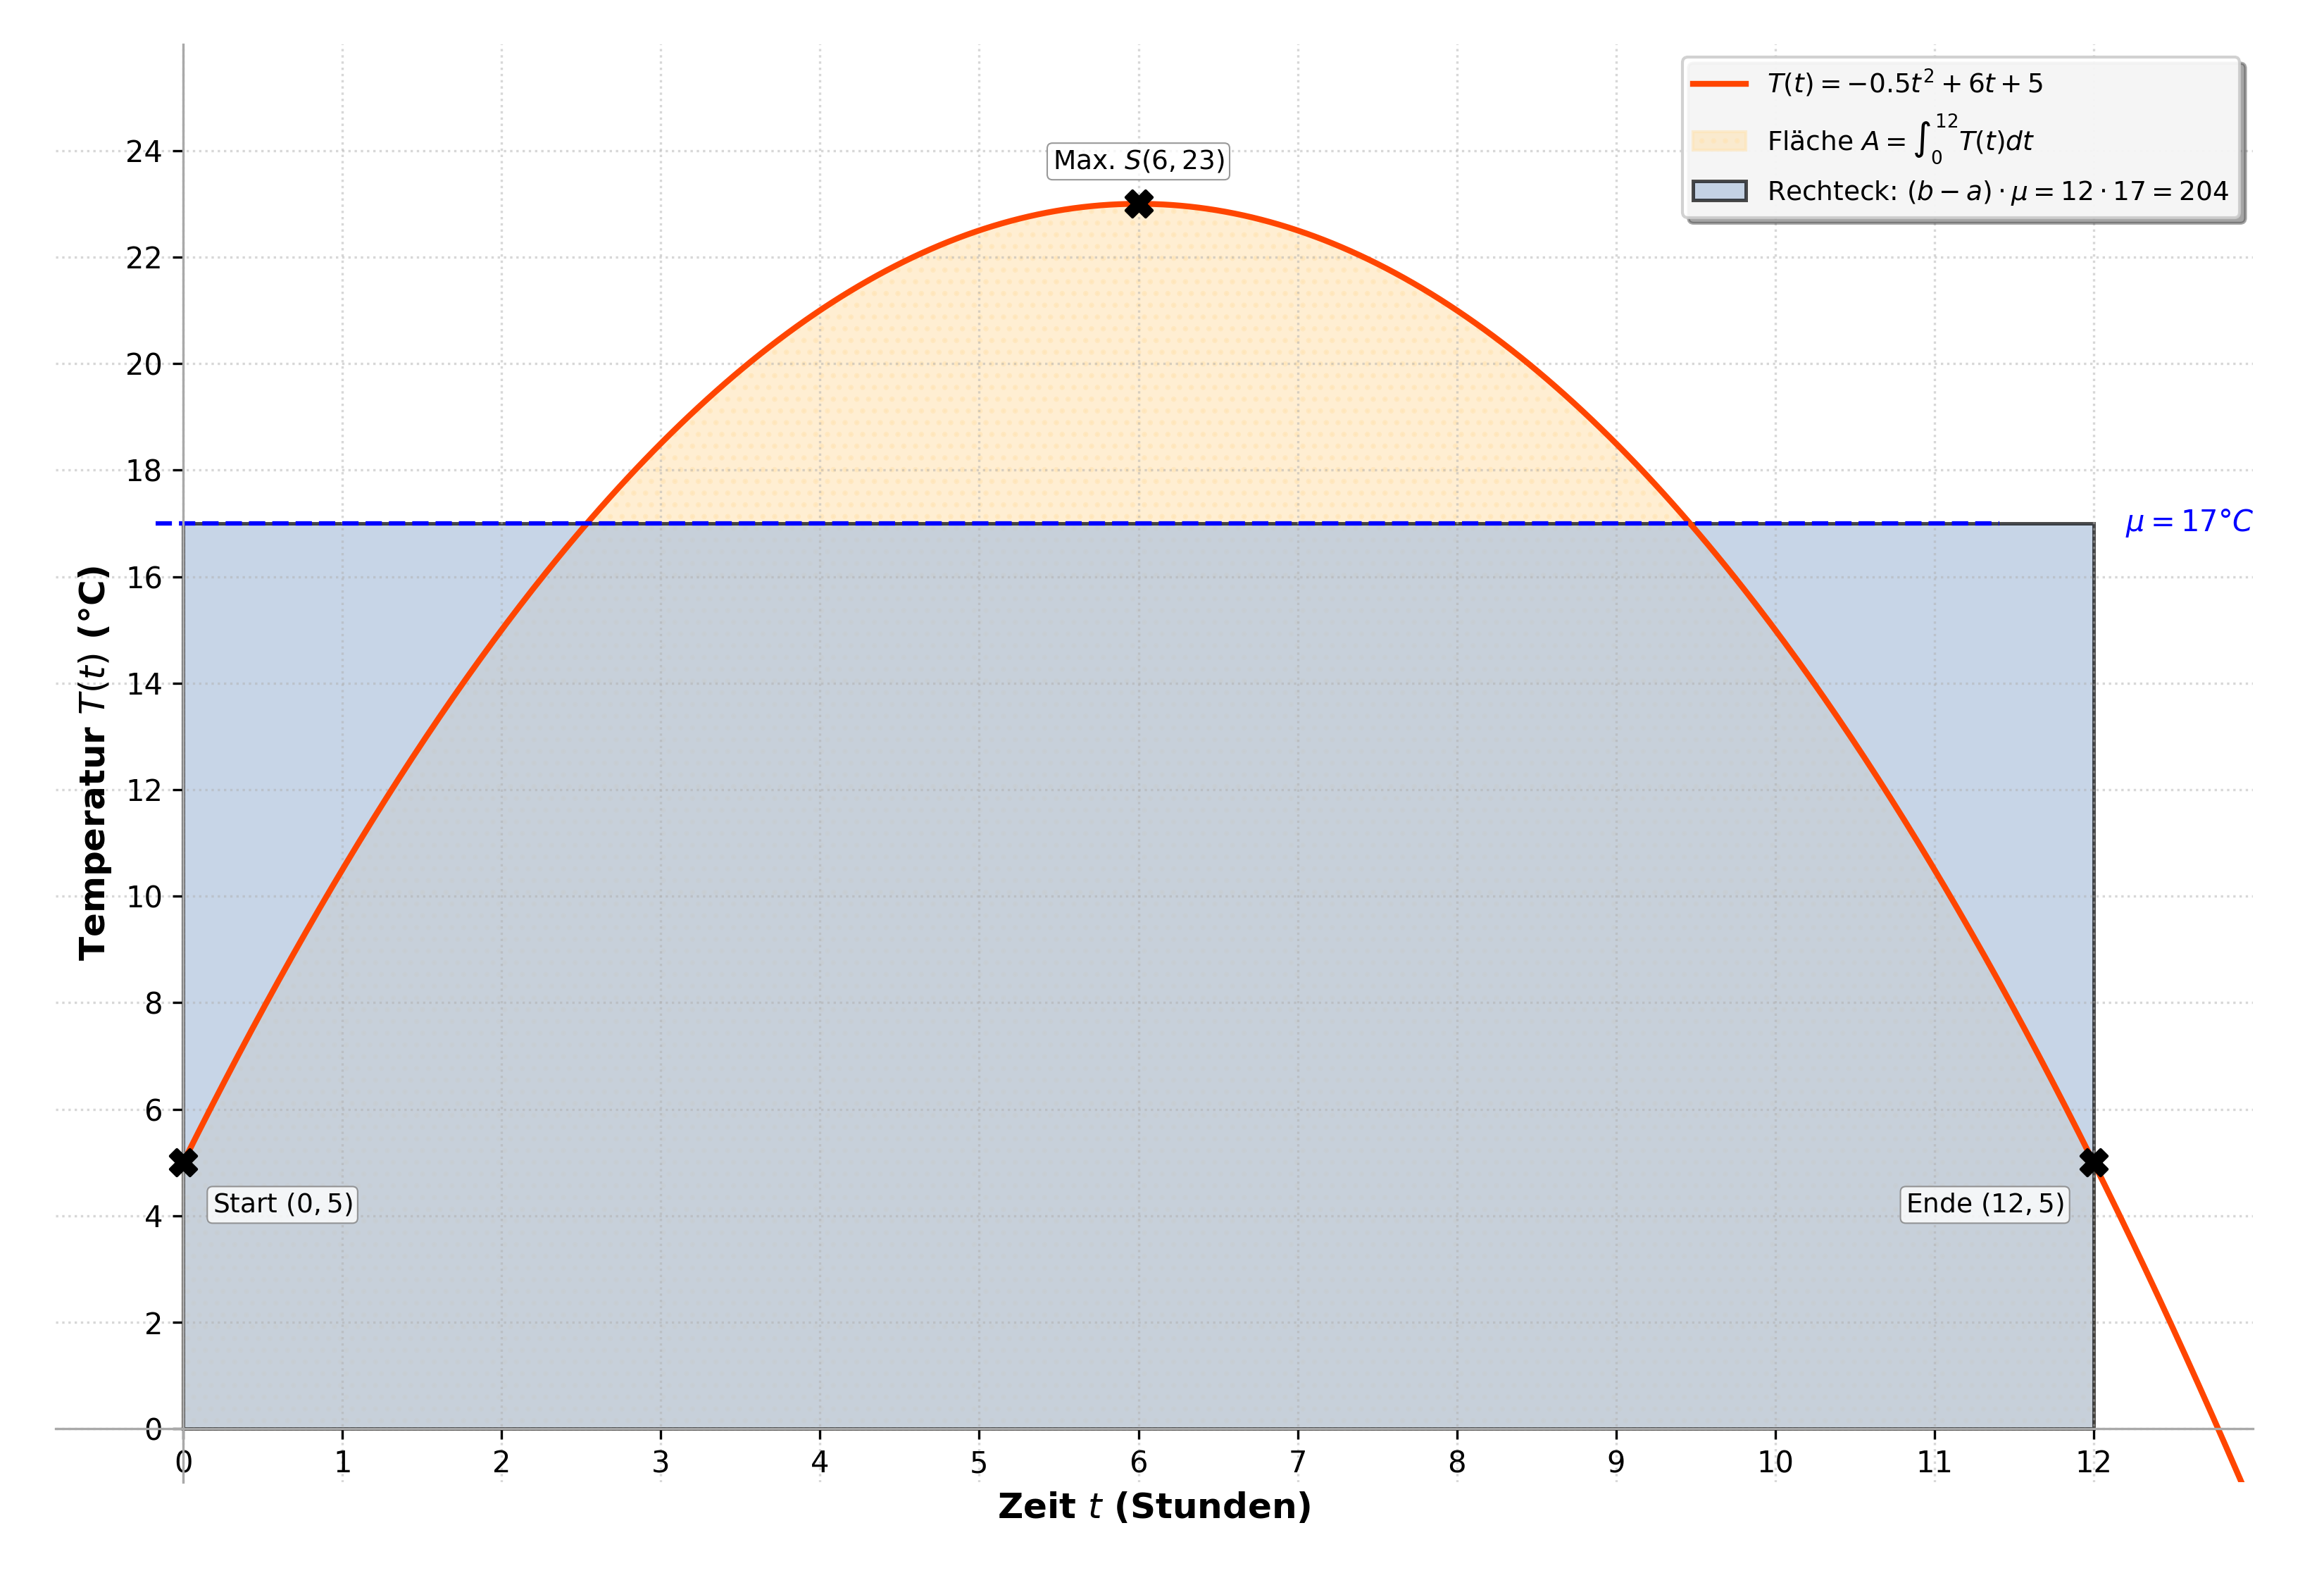
\includegraphics[width=0.8\textwidth]{grafiken/temperatur_mittelwert_skizze.png}
    % --- Beschreibung der Skizze ---
    % Die Skizze zeigt ein Koordinatensystem mit der t-Achse (Stunden, von 0 bis 12) und der T-Achse (Temperatur in °C, von ca. 0 bis 25).
    % 1. Der Graph der Funktion T(t) = -0.5t^2 + 6t + 5 ist als nach unten geöffnete Parabel eingezeichnet.
    %    - Startpunkt (0|5).
    %    - Endpunkt (12|5).
    %    - Scheitelpunkt (Maximum) S(6|23).
    % 2. Die Fläche unter dem Graphen von T(t) zwischen t=0 und t=12 ist (gedanklich oder farblich) markiert.
    % 3. Ein Rechteck ist eingezeichnet:
    %    - Es erstreckt sich auf der t-Achse von t=0 bis t=12 (Breite 12).
    %    - Seine Höhe ist die Durchschnittstemperatur mu = 17°C. Es ist also eine horizontale Linie bei T=17.
    % Die Fläche dieses Rechtecks (12 * 17 = 204) ist visuell gleich groß wie die Fläche unter der Parabelkurve T(t) von t=0 bis t=12. Bereiche der Parabel, die über das Rechteck hinausragen, werden durch Bereiche kompensiert, in denen das Rechteck über die Parabel hinausragt.
    % Die in der Aufgabenstellung referenzierte Abbildung \ref{fig:mittelwert_funktion} illustriert dieses Prinzip allgemein.
    \captionof{figure}{Graph der Temperaturfunktion $T(t)$ mit dem Rechteck des Mittelwerts $\mu=17\,$°C im Intervall $[0,12]$.}
    \label{fig:temperatur_mittelwert_skizze}
    \end{center}
    \textbf{Vergleich der Flächen:} Die Fläche des Rechtecks (Breite $12$, Höhe $17$) ist $12 \cdot 17 = 204$. Das bestimmte Integral der Temperaturfunktion über das Intervall $[0,12]$ ist ebenfalls $204$. Die Flächen sind also exakt gleich. Visuell bedeutet dies, dass der Teil der Fläche unter der Parabel, der über das Rechteck hinausragt, genauso groß ist wie der Teil der Rechteckfläche, der über die Parabel hinausragt (und somit nicht zur Fläche unter der Kurve gehört).
\end{enumerate}

\end{loesungsumgebung}

\begin{aufgabenumgebung}{Checkliste: Das bestimmte Integral – Von der Summe zur Fläche}
Das bestimmte Integral ist ein zentrales Konzept der Analysis. Diese Fragen helfen dir, die Idee dahinter besser zu greifen:

\begin{enumerate}[label=(\alph*)]
    \item \textbf{Riemannsummen als Annäherung:}
    \begin{itemize}
        \item Erkläre mit eigenen Worten, warum die Unter- und Obersumme sich dem tatsächlichen Flächeninhalt unter einer Kurve annähern, wenn man die Anzahl $n$ der Rechtecke immer weiter erhöht. Was passiert dabei mit der Breite $\Delta x$ der einzelnen Rechtecke?
        \item Skizziere eine Funktion, die in einem Intervall $[a,b]$ sowohl positive als auch negative Werte annimmt. Wie würdest du die Riemannsumme (z.B. mit linken Rändern) interpretieren? Was passiert mit den Rechtecksflächen, die unterhalb der x-Achse liegen?
    \end{itemize}
    \item \textbf{Das bestimmte Integral $\int_a^b f(x)dx$:}
    \begin{itemize}
        \item Was bedeuten die einzelnen Bestandteile der Notation: $\int$, $a$, $b$, $f(x)$ und $dx$? Welche Rolle spielt das $dx$ in Erinnerung an die Riemannsummen?
        \item Wenn $f(x)$ die Änderungsrate einer Größe beschreibt (z.B. die Geschwindigkeit $v(t)$ in m/s), welche Bedeutung und welche Einheit hat dann das bestimmte Integral $\int_{t_1}^{t_2} f(x)dx$ (bzw. $\int_{t_1}^{t_2} v(t)dt$)?
    \end{itemize}
    \item \textbf{Orientierte Fläche vs. Geometrische Fläche:}
    \begin{itemize}
        \item Angenommen, $\int_0^2 f(x)dx = 5$ und $\int_2^3 f(x)dx = -2$. Was ist der Wert von $\int_0^3 f(x)dx$? Welchen geometrischen Gesamtflächeninhalt schließt der Graph von $f(x)$ mit der x-Achse im Intervall $[0,3]$ ein? Erkläre den Unterschied.
        \item Wie würdest du vorgehen, um den \textit{geometrischen} Flächeninhalt zwischen dem Graphen von $f(x)=x^3-x$ und der x-Achse im Intervall $[-1,1]$ zu berechnen? Warum reicht hier nicht einfach $\int_{-1}^1 (x^3-x)dx$? (Tipp: Symmetrie und Nullstellen beachten).
    \end{itemize}
    \item \textbf{Eigenschaften des bestimmten Integrals:}
    \begin{itemize}
        \item Was ist der Wert von $\int_a^a f(x)dx$ und warum?
        \item Welcher Zusammenhang besteht zwischen $\int_a^b f(x)dx$ und $\int_b^a f(x)dx$? Wie lässt sich das mit $F(b)-F(a)$ erklären?
    \end{itemize}
\end{enumerate}
\end{aufgabenumgebung}

\begin{loesungsumgebung}[loes:checkliste-bestimmtes-integral]{Checkliste: Das bestimmte Integral – Von der Summe zur Fläche}

\begin{enumerate}[label=(\alph*)]
    \item \textbf{Riemannsummen als Annäherung:}
    \begin{itemize}
        \item \textbf{Annäherung an den tatsächlichen Flächeninhalt:} \\
        Wenn man die Anzahl $n$ der Rechtecke bei der Unter- oder Obersumme immer weiter erhöht, wird die Breite jedes einzelnen Rechtecks $\Delta x = \frac{b-a}{n}$ immer kleiner ($\Delta x \to 0$ für $n \to \infty$).
        Durch die kleiner werdende Breite schmiegen sich die Rechtecke immer genauer an den Verlauf der Kurve an.
        \begin{itemize}
            \item Bei der \textbf{Untersumme} werden die 'Lücken' zwischen den Rechtecken und der Kurve immer kleiner.
            \item Bei der \textbf{Obersumme} werden die 'Überstände' der Rechtecke über die Kurve immer kleiner.
        \end{itemize}
        Im Grenzwert $n \to \infty$ konvergieren sowohl die Untersumme als auch die Obersumme gegen denselben Wert, nämlich den exakten Flächeninhalt unter der Kurve (sofern die Funktion integrierbar ist). Der Fehler, der durch die Approximation mit endlich vielen Rechtecken entsteht, geht gegen Null.

        \item \textbf{Interpretation der Riemannsumme bei positiven und negativen Funktionswerten:} \\
        Betrachten wir eine Funktion, die im Intervall $[a,b]$ sowohl positive als auch negative Werte annimmt. Eine Riemannsumme (z.B. mit linken Rändern als Stützstellen $x_i^*$) ist definiert als $\sum_{i=1}^n f(x_i^*) \Delta x$.
        \begin{itemize}
            \item Liegt ein Teilintervall oberhalb der x-Achse, ist $f(x_i^*)$ positiv, und der Term $f(x_i^*) \Delta x$ entspricht dem (positiven) Flächeninhalt des Rechtecks.
            \item Liegt ein Teilintervall unterhalb der x-Achse, ist $f(x_i^*)$ negativ, und der Term $f(x_i^*) \Delta x$ entspricht dem \textit{negativen} Wert des Flächeninhalts des Rechtecks.
        \end{itemize}
        Die Riemannsumme ist also die Summe dieser vorzeichenbehafteten Flächenbeiträge. Sie stellt die \textbf{orientierte Fläche} (oder Flächenbilanz) zwischen dem Graphen und der x-Achse dar. Flächenstücke oberhalb der x-Achse gehen positiv, Flächenstücke unterhalb der x-Achse negativ in die Summe ein.
        \begin{center}
        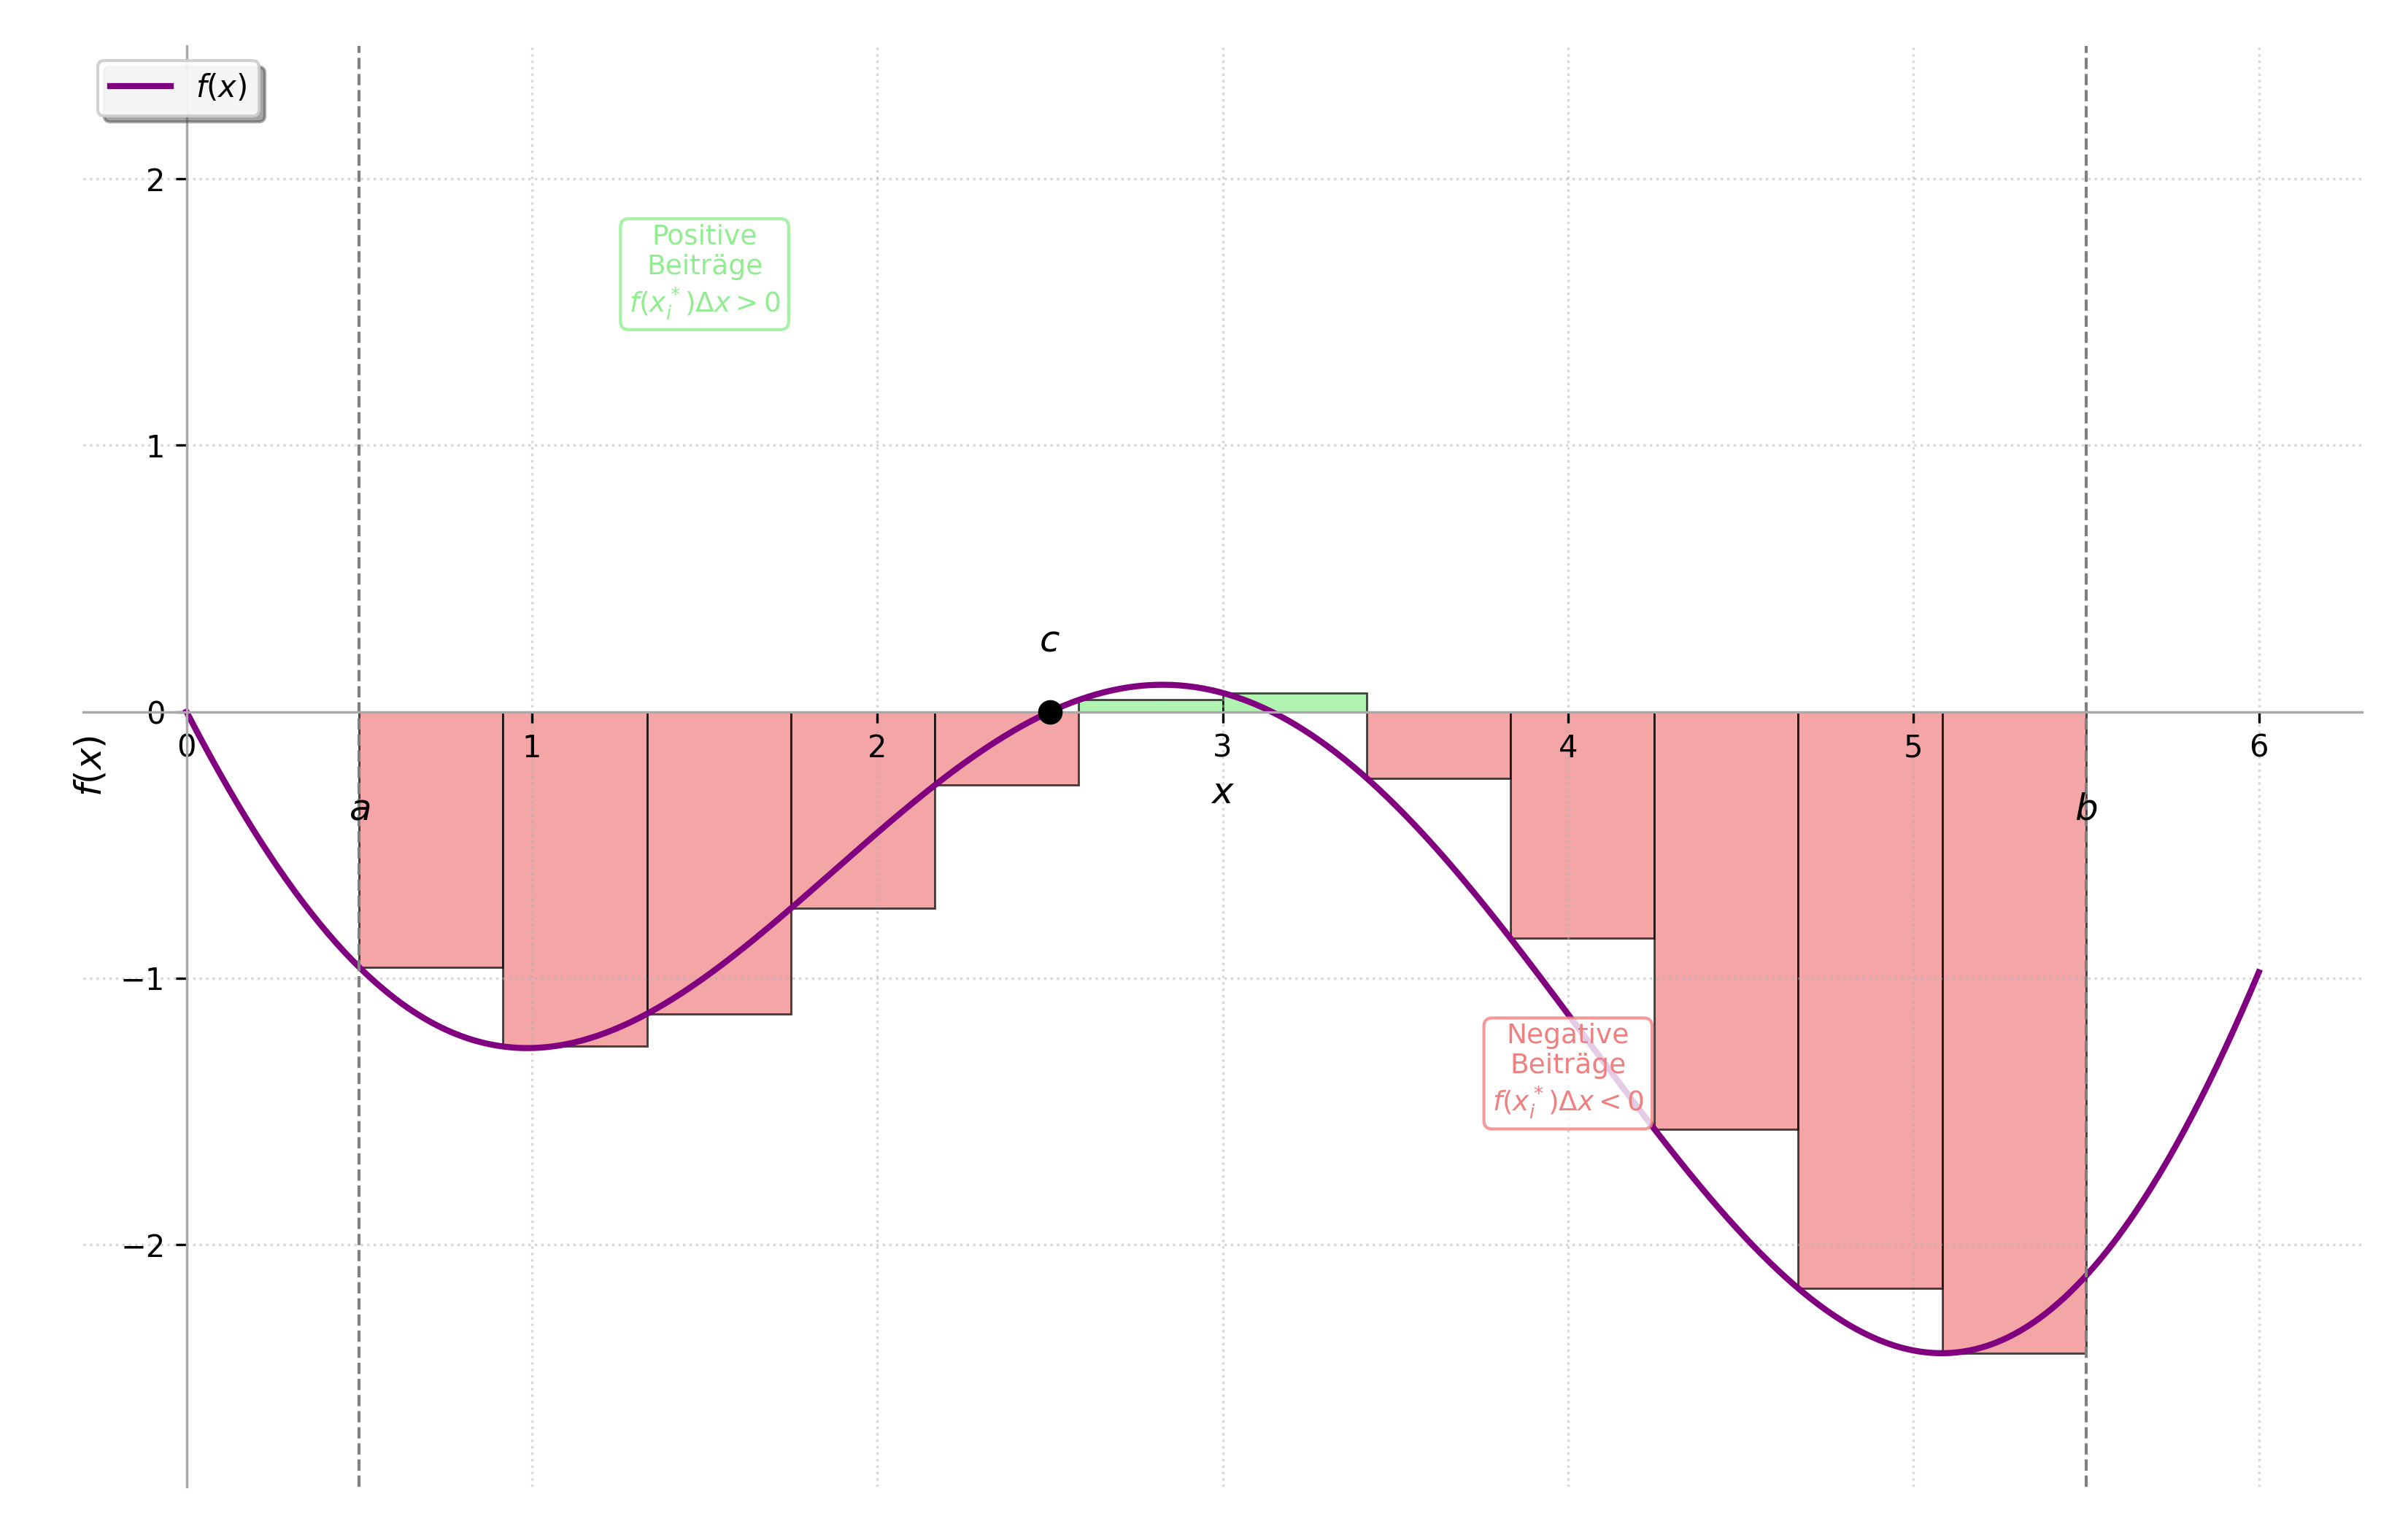
\includegraphics[width=0.8\textwidth]{grafiken/riemann_positiv_negativ.png}
        % --- Beschreibung der Skizze ---
        % Die Skizze zeigt eine Funktion f(x) im Intervall [a,b].
        % Ein Teil des Graphen (z.B. von a bis c) verläuft oberhalb der x-Achse. Die Riemann-Rechtecke hier haben positive Flächenbeiträge.
        % Ein anderer Teil des Graphen (z.B. von c bis b) verläuft unterhalb der x-Achse. Die Riemann-Rechtecke hier haben negative Flächenbeiträge (sind nach unten gezeichnet).
        \captionof{figure}{Interpretation der Riemannsumme bei positiven und negativen Funktionswerten.}
        \label{fig:riemann_positiv_negativ}
        \end{center}
    \end{itemize}

    \item \textbf{Das bestimmte Integral $\int_a^b f(x)dx$:}
    \begin{itemize}
        \item \textbf{Bedeutung der Notation:}
        \begin{itemize}
            \item $\mathbf{\int}$: Das Integralzeichen. Es ist ein stilisiertes 'S' und steht für 'Summe', da das Integral der Grenzwert einer Summe (der Riemannsumme) ist.
            \item $\mathbf{a}$: Die untere Integrationsgrenze. Sie gibt den Startpunkt des Intervalls an, über das integriert wird.
            \item $\mathbf{b}$: Die obere Integrationsgrenze. Sie gibt den Endpunkt des Intervalls an.
            \item $\mathbf{f(x)}$: Der Integrand. Dies ist die Funktion, deren Fläche unter dem Graphen (bzw. deren orientierte Fläche) berechnet wird. Sie gibt die 'Höhe' der infinitesimalen Streifen an.
            \item $\mathbf{dx}$: Das Differential. Es gibt an, nach welcher Variablen integriert wird (hier $x$). Es symbolisiert eine infinitesimal kleine Breite eines Rechteckstreifens und erinnert an das $\Delta x$ aus den Riemannsummen, wobei $dx = \lim_{n \to \infty} \Delta x$.
        \end{itemize}
        \item \textbf{Bedeutung des Integrals einer Änderungsrate:}
        Wenn $f(x)$ die Änderungsrate einer Größe $G(x)$ beschreibt (d.h. $f(x) = G'(x)$), dann ist das bestimmte Integral $\int_{t_1}^{t_2} f(x)dx$ (oder, mit Variable $t$, $\int_{t_1}^{t_2} v(t)dt$) die \textbf{Gesamtänderung der Größe $G(x)$ im Intervall $[t_1, t_2]$}. Nach dem Hauptsatz der Differential- und Integralrechnung ist dies $G(t_2) - G(t_1)$.
        Beispiel: Ist $v(t)$ die Geschwindigkeit eines Objekts in m/s, so ist $\int_{t_1}^{t_2} v(t)dt$ die im Zeitintervall $[t_1, t_2]$ zurückgelegte Strecke (genauer: die Änderung der Position, also die Verschiebung) in Metern. Die Einheit des Integrals ist das Produkt der Einheit von $f(x)$ (oder $v(t)$) und der Einheit von $x$ (oder $t$). (z.B. $\frac{m}{s} \cdot s = m$).
    \end{itemize}

    \item \textbf{Orientierte Fläche vs. Geometrische Fläche:}
    \begin{itemize}
        \item Angenommen, $\int_0^2 f(x)dx = 5$ und $\int_2^3 f(x)dx = -2$.
        Der Wert von $\int_0^3 f(x)dx$ ist aufgrund der Additivität von Intervallen:
        $$ \int_0^3 f(x)dx = \int_0^2 f(x)dx + \int_2^3 f(x)dx = 5 + (-2) = \mathbf{3} $$
        Dies ist die \textbf{orientierte Gesamtfläche}.
        Der \textbf{geometrische Gesamtflächeninhalt} $A_{geom}$ im Intervall $[0,3]$ ist die Summe der Beträge der Flächenanteile:
        $A_{geom} = \left| \int_0^2 f(x)dx \right| + \left| \int_2^3 f(x)dx \right| = |5| + |-2| = 5 + 2 = \mathbf{7}$.
        \textit{Unterschied:} Das bestimmte Integral $\int_0^3 f(x)dx=3$ ist die Flächenbilanz, bei der die Fläche unter der x-Achse (Wert -2) von der Fläche über der x-Achse (Wert 5) abgezogen wird. Der geometrische Flächeninhalt von 7 ist die Summe der tatsächlichen (positiven) Flächengrößen, unabhängig davon, ob sie ober- oder unterhalb der x-Achse liegen.

        \item \textbf{Geometrischer Flächeninhalt für $f(x)=x^3-x$ im Intervall $[-1,1]$:}
        Die Funktion $f(x)=x^3-x = x(x-1)(x+1)$ hat Nullstellen bei $x_1=-1, x_2=0, x_3=1$.
        Sie ist punktsymmetrisch zum Ursprung ($f(-x)=-f(x)$). Daher ist $\int_{-1}^1 (x^3-x)dx = 0$. Dies ist die orientierte Fläche, nicht der geometrische Flächeninhalt.
        Um den geometrischen Flächeninhalt zu berechnen, müssen wir die Beträge der Integrale über die Teilintervalle addieren, in denen die Funktion unterschiedliche Vorzeichen hat:
        \begin{itemize}
            \item Im Intervall $[-1,0]$: z.B. $f(-0.5) = (-0.5)^3 - (-0.5) = -0.125 + 0.5 = 0.375 > 0$. Also $f(x) \ge 0$.
            \item Im Intervall $[0,1]$: z.B. $f(0.5) = (0.5)^3 - (0.5) = 0.125 - 0.5 = -0.375 < 0$. Also $f(x) \le 0$.
        \end{itemize}
        Der geometrische Flächeninhalt $A_{geom}$ ist:
        $A_{geom} = \int_{-1}^0 (x^3-x)dx + \left| \int_0^1 (x^3-x)dx \right| = \int_{-1}^0 (x^3-x)dx - \int_0^1 (x^3-x)dx$.
        Eine Stammfunktion ist $F(x) = \frac{1}{4}x^4 - \frac{1}{2}x^2$.
        $\int_{-1}^0 (x^3-x)dx = [F(x)]_{-1}^0 = F(0) - F(-1) = 0 - (\frac{1}{4}(-1)^4 - \frac{1}{2}(-1)^2) = -(\frac{1}{4}-\frac{1}{2}) = -(-\frac{1}{4}) = \frac{1}{4}$.
        $\int_0^1 (x^3-x)dx = [F(x)]_0^1 = F(1) - F(0) = (\frac{1}{4}(1)^4 - \frac{1}{2}(1)^2) - 0 = \frac{1}{4}-\frac{1}{2} = -\frac{1}{4}$.
        $A_{geom} = \frac{1}{4} + |-\frac{1}{4}| = \frac{1}{4} + \frac{1}{4} = \mathbf{\frac{1}{2}}$.
        (Aufgrund der Punktsymmetrie ist $A_{geom} = 2 \cdot \int_{-1}^0 (x^3-x)dx = 2 \cdot \frac{1}{4} = \frac{1}{2}$).
    \end{itemize}

    \item \textbf{Eigenschaften des bestimmten Integrals:}
    \begin{itemize}
        \item \textbf{Wert von $\int_a^a f(x)dx$ und warum?}
        Der Wert ist $\mathbf{0}$.
        \textit{Begründung:} Die Integrationsgrenzen sind identisch, d.h. die Breite des Integrationsintervalls ist $b-a = a-a = 0$. Eine Fläche der Breite Null hat den Inhalt Null.
        Mit dem Hauptsatz: $\int_a^a f(x)dx = F(a) - F(a) = 0$.

        \item \textbf{Zusammenhang zwischen $\int_a^b f(x)dx$ und $\int_b^a f(x)dx$?}
        Es gilt: $\mathbf{\int_a^b f(x)dx = -\int_b^a f(x)dx}$.
        \textit{Erklärung mit $F(b)-F(a)$:}
        $\int_a^b f(x)dx = F(b) - F(a)$.
        $\int_b^a f(x)dx = F(a) - F(b)$.
        Da $F(b) - F(a) = -(F(a) - F(b))$, folgt die Beziehung. Das Vertauschen der Integrationsgrenzen kehrt das Vorzeichen des Integralwerts um.
    \end{itemize}
\end{enumerate}

\end{loesungsumgebung}

\begin{aufgabenumgebung}{Checkliste: Stammfunktion und Hauptsatz – Die große Verbindung}
Die Entdeckung des Zusammenhangs zwischen Ableitung und Integral durch den Hauptsatz ist revolutionär. Teste dein Verständnis:

\begin{enumerate}[label=(\alph*)]
    \item \textbf{Stammfunktion und unbestimmtes Integral:}
    \begin{itemize}
        \item Erkläre den Unterschied zwischen 'einer Stammfunktion $F(x)$ von $f(x)$' und 'dem unbestimmten Integral $\int f(x)dx$'. Warum ist die Integrationskonstante $C$ beim unbestimmten Integral so wichtig?
        \item Wenn $F(x)$ eine Stammfunktion von $f(x)$ ist und $G(x)$ eine Stammfunktion von $g(x)$ ist: Ist $F(x) \cdot G(x)$ dann automatisch eine Stammfunktion von $f(x) \cdot g(x)$? Überprüfe deine Vermutung mit einem einfachen Beispiel (z.B. $f(x)=1, g(x)=2x$). Was schließt du daraus für Integrationsregeln für Produkte?
    \end{itemize}
    \item \textbf{Der Hauptsatz der Differential- und Integralrechnung (HDI):}
    \begin{itemize}
        \item Formuliere den HDI mit eigenen Worten. Was ist die 'Brücke', die er zwischen der Differential- und Integralrechnung schlägt?
        \item Warum ist der HDI so praktisch für die Berechnung von bestimmten Integralen im Vergleich zur Methode mit den Riemannsummen?
        \item Angenommen, jemand behauptet, eine Stammfunktion von $f(x)=2x$ sei $F(x)=x^2+1000$, und eine andere Person sagt, es sei $G(x)=x^2-5$. Wer hat Recht? Und wie wirkt sich die Wahl von $F(x)$ oder $G(x)$ auf das Ergebnis von $\int_1^2 2x \,dx$ aus? Begründe.
    \end{itemize}
    \item \textbf{Anwendungen und Interpretationen:}
    \begin{itemize}
        \item Wenn $\int_a^b f(x)dx = 0$ ist, bedeutet das zwangsläufig, dass $f(x)=0$ für alle $x \in [a,b]$ gilt? Erkläre anhand einer Skizze oder eines Beispiels (nutze Symmetrie!).
        \item Erkläre die geometrische Bedeutung des Mittelwerts $\mu = \frac{1}{b-a} \int_a^b f(x)dx$ einer Funktion $f(x)$ im Intervall $[a,b]$ mithilfe eines flächengleichen Rechtecks.
    \end{itemize}
\end{enumerate}
\end{aufgabenumgebung}

\begin{loesungsumgebung}[loes:checkliste-hdi-stammfunktion]{Checkliste: Stammfunktion und Hauptsatz – Die große Verbindung}

\begin{enumerate}[label=(\alph*)]
    \item \textbf{Stammfunktion und unbestimmtes Integral:}
    \begin{itemize}
        \item \textbf{Unterschied und Wichtigkeit der Konstante $C$:}
        \begin{itemize}
            \item \textbf{Eine Stammfunktion $F(x)$ von $f(x)$:} Dies ist eine \textit{spezifische} Funktion, deren Ableitung $F'(x)$ gleich der ursprünglichen Funktion $f(x)$ ist. Zum Beispiel ist $F(x) = x^2$ eine Stammfunktion von $f(x)=2x$, da $(x^2)' = 2x$.
            \item \textbf{Das unbestimmte Integral $\int f(x)dx$:} Dies bezeichnet die \textit{Menge aller} Stammfunktionen von $f(x)$. Da sich zwei beliebige Stammfunktionen derselben Funktion nur durch eine additive Konstante unterscheiden ($F_1'(x) = f(x)$ und $F_2'(x) = f(x) \implies (F_1(x)-F_2(x))' = 0 \implies F_1(x)-F_2(x)=C$), schreibt man $\int f(x)dx = F(x) + C$. Hierbei ist $F(x)$ irgendeine partikulare Stammfunktion und $C$ die Integrationskonstante (eine beliebige reelle Zahl). Für $f(x)=2x$ ist $\int 2x dx = x^2 + C$.
            \item \textbf{Wichtigkeit von $C$:} Die Integrationskonstante $C$ ist entscheidend, da sie die gesamte Familie von Funktionen darstellt, die beim Ableiten $f(x)$ ergeben. Diese Funktionen sind Graphen, die sich nur durch eine Verschiebung in y-Richtung unterscheiden. Beim Berechnen \textit{bestimmter} Integrale ($F(b)-F(a)$) fällt die Konstante $C$ heraus, da $(F(b)+C) - (F(a)+C) = F(b)-F(a)$. Aber für das allgemeine Konzept der Stammfunktion und z.B. beim Lösen von Differentialgleichungen ist $C$ unerlässlich.
        \end{itemize}

        \item \textbf{Ist $F(x) \cdot G(x)$ eine Stammfunktion von $f(x) \cdot g(x)$?}
        Die Vermutung ist: \textbf{Nein}, im Allgemeinen nicht.
        Zur Überprüfung leiten wir $F(x) \cdot G(x)$ mit der Produktregel ab:
        $(F(x) \cdot G(x))' = F'(x) \cdot G(x) + F(x) \cdot G'(x)$.
        Da $F'(x)=f(x)$ und $G'(x)=g(x)$, erhalten wir:
        $(F(x) \cdot G(x))' = f(x)G(x) + F(x)g(x)$.
        Dies ist im Allgemeinen nicht gleich $f(x)g(x)$.
        \textit{Beispiel:} Sei $f(x)=1$ und $g(x)=2x$.
        Dann ist eine Stammfunktion $F(x)=x$ und eine Stammfunktion $G(x)=x^2$.
        Das Produkt der Funktionen ist $f(x)g(x) = 1 \cdot 2x = 2x$.
        Das Produkt der Stammfunktionen ist $F(x)G(x) = x \cdot x^2 = x^3$.
        Die Ableitung von $F(x)G(x)$ ist $(x^3)' = 3x^2$.
        Da $3x^2 \neq 2x$ (außer für spezielle $x$), ist $F(x)G(x)$ keine Stammfunktion von $f(x)g(x)$.
        \textit{Schlussfolgerung:} Es gibt keine einfache 'Produktregel' für die Integration in der Form $\int f(x)g(x)dx = (\int f(x)dx)(\int g(x)dx)$. Methoden wie die partielle Integration werden für das Integrieren von Produkten benötigt.
    \end{itemize}

    \item \textbf{Der Hauptsatz der Differential- und Integralrechnung (HDI):}
    \begin{itemize}
        \item \textbf{HDI in eigenen Worten und die 'Brücke':}
        Der Hauptsatz schlägt die fundamentale 'Brücke' zwischen der Differentialrechnung (dem Studium von Änderungsraten und Ableitungen) und der Integralrechnung (ursprünglich dem Studium von Flächeninhalten). Er besagt im Wesentlichen zwei Dinge:
        \begin{enumerate}
            \item Die Ableitung einer über eine variable obere Grenze definierten Integralfunktion $\Phi(x) = \int_a^x f(t)dt$ ist die ursprüngliche Funktion $f(x)$ selbst (also $\Phi'(x) = f(x)$). Das zeigt, dass Integration die Umkehroperation zur Differentiation ist.
            \item Das bestimmte Integral $\int_a^b f(x)dx$ (das die orientierte Fläche unter dem Graphen von $f(x)$ von $a$ bis $b$ darstellt) kann berechnet werden, indem man eine beliebige Stammfunktion $F(x)$ von $f(x)$ findet und die Differenz $F(b) - F(a)$ bildet.
        \end{enumerate}
        Die 'Brücke' besteht also darin, dass die Berechnung von Flächen (Integralrechnung) auf das Finden von Stammfunktionen (Umkehrung der Differentialrechnung) zurückgeführt wird.

        \item \textbf{Praktischer Nutzen des HDI im Vergleich zu Riemannsummen:}
        Die Berechnung bestimmter Integrale über den Grenzwert von Riemannsummen ist oft sehr komplex und langwierig. Der HDI bietet eine wesentlich einfachere und oft exakte algebraische Methode: Finde eine Stammfunktion $F(x)$ (was oft mit bekannten Integrationsregeln möglich ist) und werte $F(b)-F(a)$ aus. Dies ist in der Praxis erheblich effizienter.

        \item \textbf{Stammfunktionen $F(x)=x^2+1000$ und $G(x)=x^2-5$ für $f(x)=2x$:}
        Beide Personen haben Recht.
        $(x^2+1000)' = 2x + 0 = 2x$.
        $(x^2-5)' = 2x + 0 = 2x$.
        Sowohl $F(x)$ als auch $G(x)$ sind gültige Stammfunktionen von $f(x)=2x$, da sie sich nur um eine Konstante unterscheiden.
        \textit{Auswirkung auf $\int_1^2 2x \,dx$:}
        Mit $F(x)$: $\int_1^2 2x \,dx = [x^2+1000]_1^2 = (2^2+1000) - (1^2+1000) = (4+1000) - (1+1000) = 1004 - 1001 = 3$.
        Mit $G(x)$: $\int_1^2 2x \,dx = [x^2-5]_1^2 = (2^2-5) - (1^2-5) = (4-5) - (1-5) = -1 - (-4) = -1+4 = 3$.
        Das Ergebnis des bestimmten Integrals ist in beiden Fällen $\mathbf{3}$. Dies liegt daran, dass sich die additive Konstante $C$ bei der Differenzbildung $F(b)-F(a)$ heraushebt: $(F_0(b)+C) - (F_0(a)+C) = F_0(b)-F_0(a)$. Die Wahl der spezifischen Stammfunktion (d.h. der Wert von $C$) beeinflusst den Wert des bestimmten Integrals nicht.
    \end{itemize}

    \item \textbf{Anwendungen und Interpretationen:}
    \begin{itemize}
        \item \textbf{Bedeutung von $\int_a^b f(x)dx = 0$:}
        Nein, das bedeutet \textbf{nicht zwangsläufig}, dass $f(x)=0$ für alle $x \in [a,b]$ gilt.
        Das bestimmte Integral stellt die \textit{orientierte} Fläche dar. Ein Wert von Null bedeutet, dass sich die Flächenanteile oberhalb der x-Achse und die Flächenanteile unterhalb der x-Achse exakt ausgleichen (kompensieren).
        \textit{Beispiel:} Für $f(x)=x$ im Intervall $[-1,1]$ gilt $\int_{-1}^1 x \,dx = [\frac{1}{2}x^2]_{-1}^1 = \frac{1}{2} - \frac{1}{2} = 0$. Die Funktion $f(x)=x$ ist jedoch im Intervall nicht überall Null. Die Fläche des Dreiecks unter der x-Achse von $x=-1$ bis $x=0$ ist $-\frac{1}{2}$, und die Fläche des Dreiecks über der x-Achse von $x=0$ bis $x=1$ ist $+\frac{1}{2}$. Die Summe ist $0$.
        \begin{center}
        % 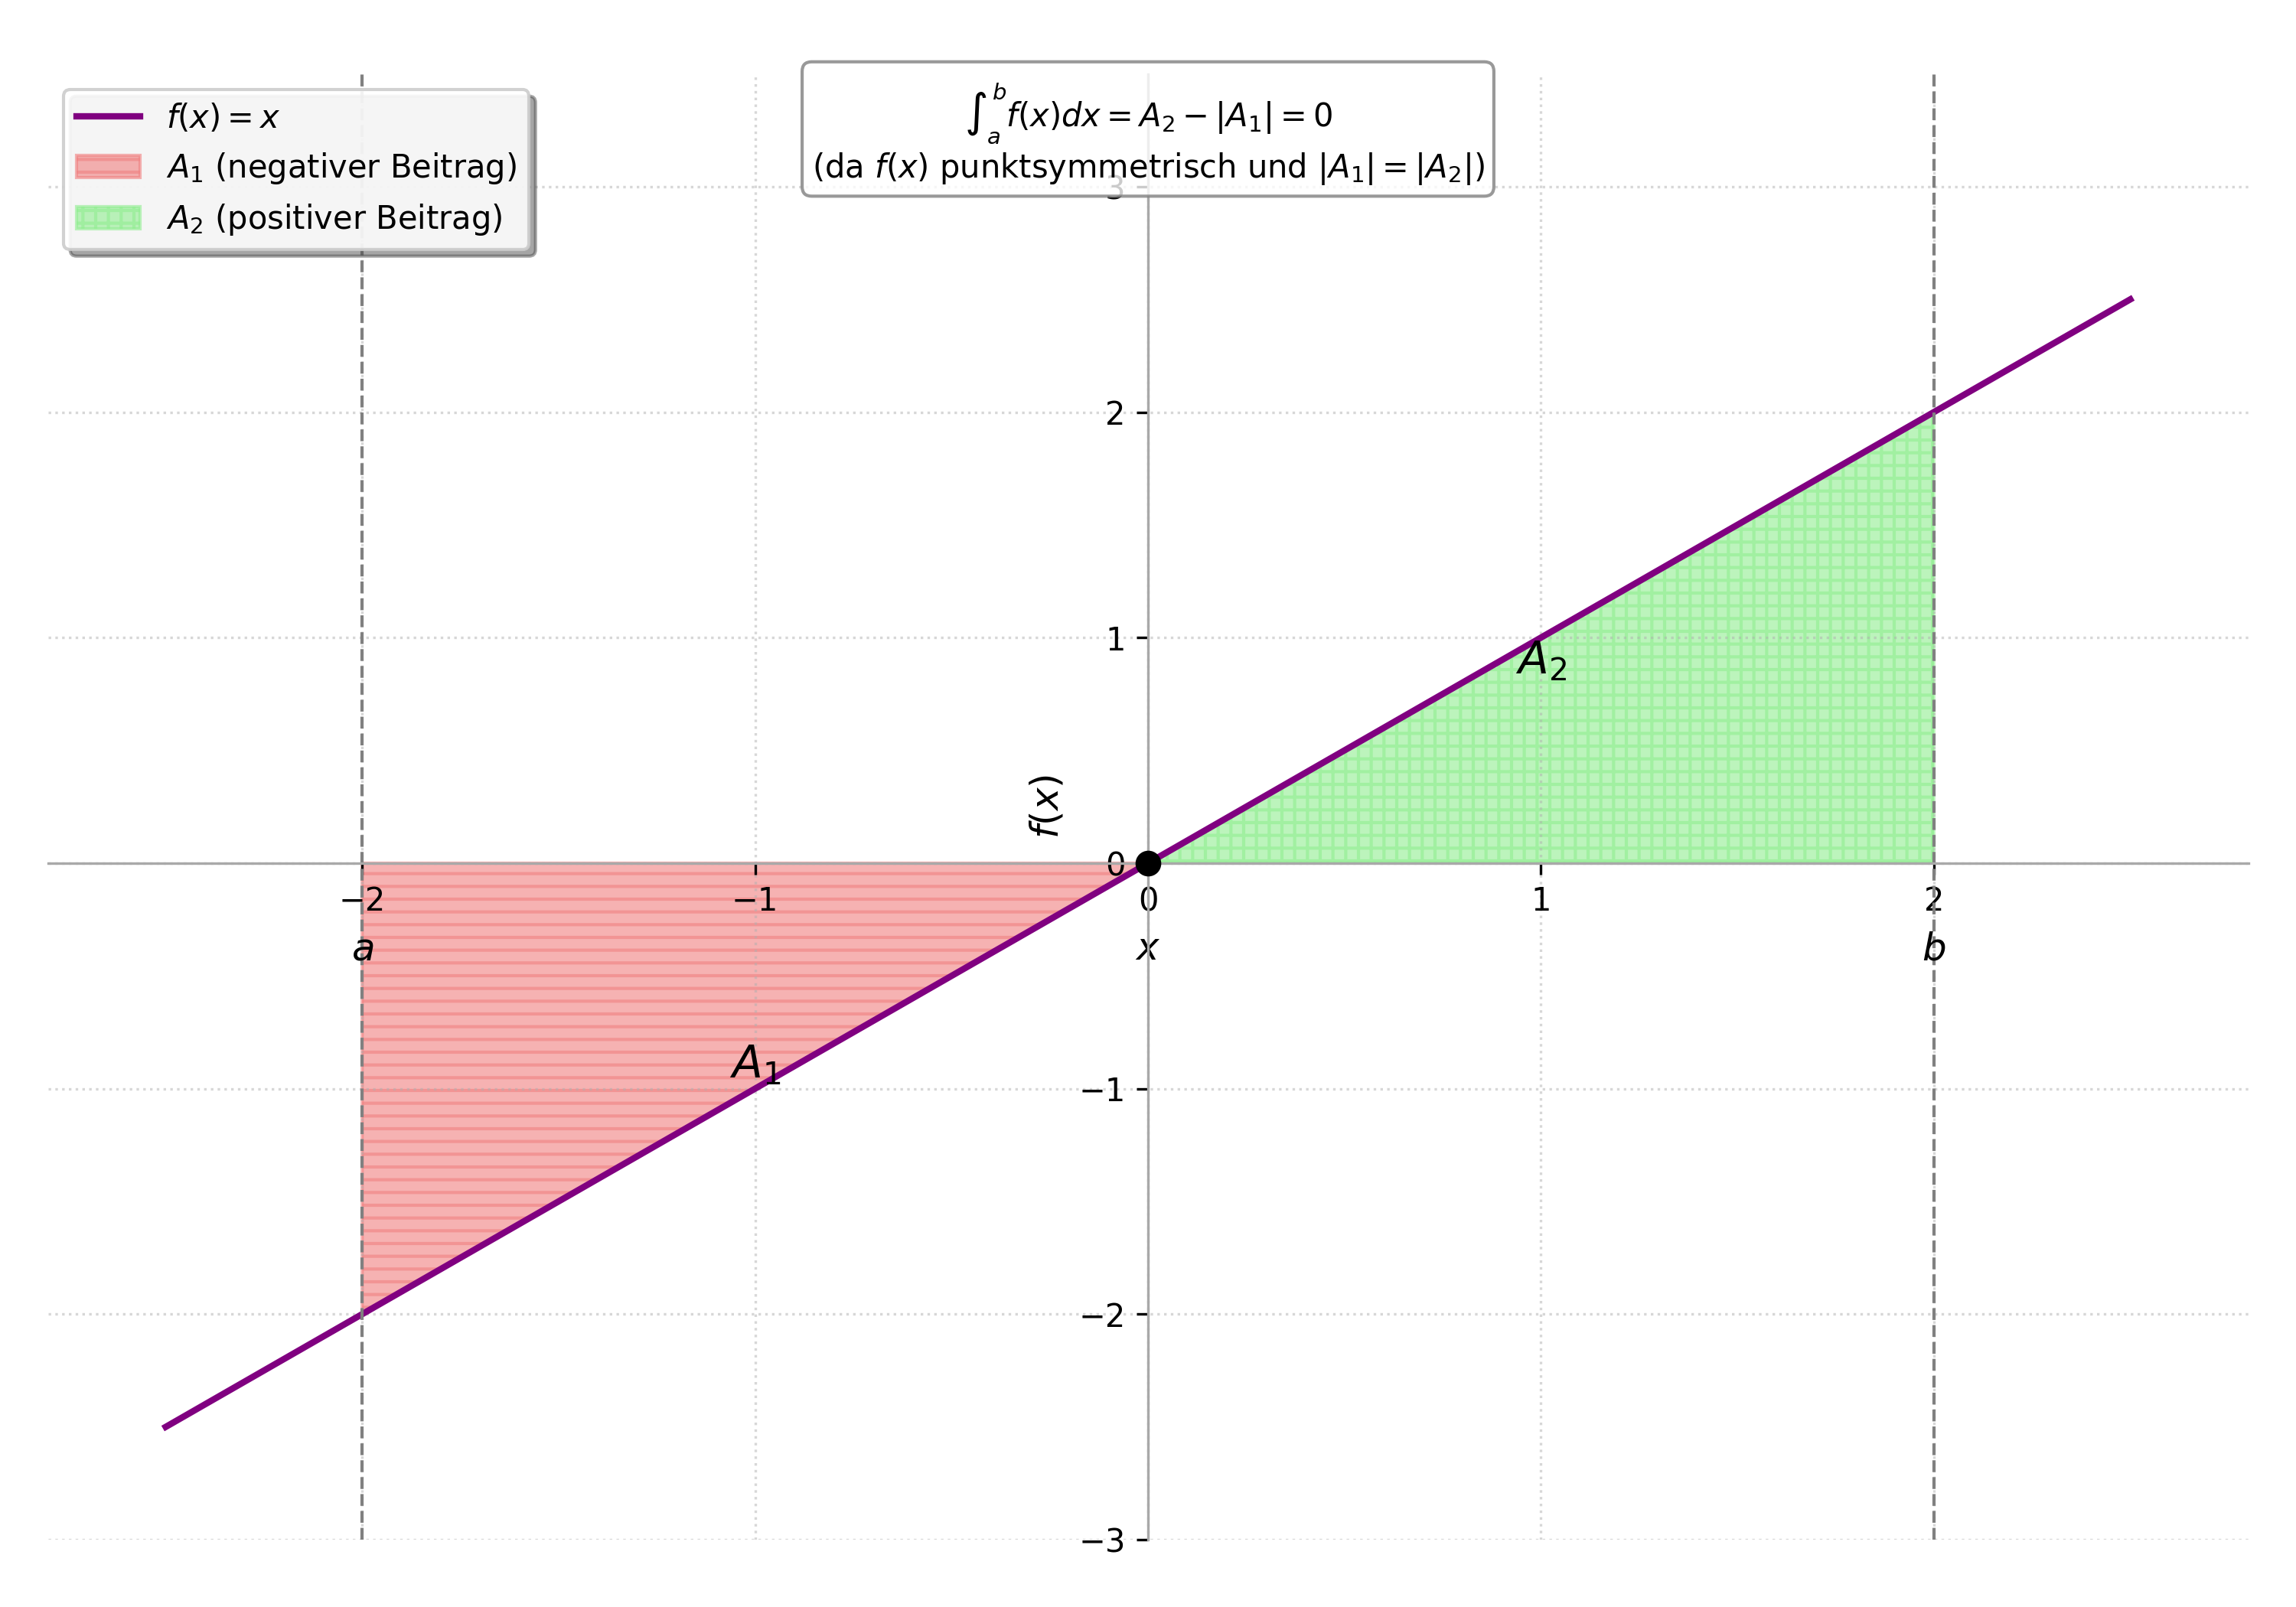
\includegraphics[width=0.8\textwidth]{grafiken/integral_null_flaeche.png}
        % --- Beschreibung der Skizze ---
        % Die Skizze zeigt eine Funktion (z.B. f(x)=x oder eine Sinuswelle über eine Periode), die im Intervall [a,b] sowohl positive als auch negative Funktionswerte annimmt.
        % Die Flächenstücke oberhalb der x-Achse sind schraffiert und als A1, A3,... bezeichnet.
        % Die Flächenstücke unterhalb der x-Achse sind schraffiert und als A2, A4,... bezeichnet.
        % Das Integral ist Null, wenn die Summe der positiv gewerteten Flächen gleich der Summe der negativ gewerteten Flächen ist (z.B. A1 - A2 + A3 = 0).
        \captionof{figure}{Beispiel für $\int_a^b f(x)dx = 0$ obwohl $f(x) \not\equiv 0$.}
        \label{fig:integral_null_flaeche}
        \end{center}

        \item \textbf{Geometrische Bedeutung des Mittelwerts $\mu = \frac{1}{b-a} \int_a^b f(x)dx$:}
        Der Mittelwert $\mu$ einer Funktion $f(x)$ im Intervall $[a,b]$ ist die Höhe eines Rechtecks, dessen Grundseite die Länge des Intervalls $(b-a)$ hat und dessen Flächeninhalt $\mu \cdot (b-a)$ gleich dem orientierten Flächeninhalt $\int_a^b f(x)dx$ unter dem Graphen von $f(x)$ ist.
        Anschaulich gesprochen: Wenn man sich die Fläche $\int_a^b f(x)dx$ als eine Art 'Gebirge und Täler' vorstellt, dann ist $\mu$ die durchschnittliche Höhe dieses Geländes über der Breite $(b-a)$. Das Rechteck mit der Höhe $\mu$ und der Breite $(b-a)$ hat exakt denselben (orientierten) Flächeninhalt wie die Fläche unter der Kurve von $f(x)$ im Intervall $[a,b]$.
    \end{itemize}
\end{enumerate}

\end{loesungsumgebung}